\documentclass[BCOR=12mm,DIV11,titlepage,a4paper,oneside]{scrbook}

% package for encoding, here UTF-8
\usepackage[utf8]{inputenc}

% package for including graphics with figure-environment
\usepackage{graphicx}

% package for changing header and footer
\usepackage{fancyhdr}
% Uses the package for own page style
\pagestyle{fancy}
% Creates a line in header (to hide this, change to 0.0pt)
\renewcommand*{\headrulewidth}{0.4pt}
\fancyhf{}
\fancyhead[EC,OC]{\thepage}
% \fancyhead[EL]{\leftmark}
% \fancyhead[OR]{\rightmark}
% \fancyhead[ER,OL]{\thepage}
\renewcommand{\sectionmark}[1]{
\markboth{\thechapter{} #1}{\thechapter{} #1}
}

% changes page numbering of table of content with own style
\renewcommand*{\indexpagestyle}{fancy}
% prevents page numbering on "Part" pages
\renewcommand*{\partpagestyle}{empty}
% changes page numbering of chapters with own style
\renewcommand*{\chapterpagestyle}{fancy}

% Changes numbering of figures (chapter-dependent, e.g. figure 1.1)
\renewcommand*{\thefigure}{\thechapter.\arabic{figure}}
% Changes numbering of tables (table-depentent, e.g. table 1.1)
\renewcommand*{\thetable}{\thechapter.\arabic{table}}

% prevents indent after section and figures
\setlength{\parindent}{0pt}

% prevents that a new page is created for a single word / row
\clubpenalty = 10000 % exclusion of orphans
\widowpenalty = 10000 % exclusion of widow lines

% package for bibliography
\usepackage[authoryear,round]{natbib}
\bibliographystyle{natdin}

% package for the use of URL by the use of the command \url{}
\usepackage{url}

% package for line spacing (onehalfspace, singlespace)
\usepackage{setspace}

% package for the creation of quotation marks by the use of the command \enquote{Text}
\usepackage[english]{babel}
\usepackage[babel, german=quotes]{csquotes}

% package for colored text
% black,white,green,red,blue,yellow,cyan,magenta
\usepackage{color}

% package for colored tables
\usepackage{colortbl}

% Rotation of floating objects (figures, tables, etc.)
\usepackage{rotating}

% Rotation of single pages by the use of the command begin{landscape}
\usepackage{lscape}

% package for colored background Verbatim-environment (source code environment)
\usepackage{fancyvrb}
\usepackage{verbatim,moreverb}
% defindes shade of grey for source code environment 80 % grey
\definecolor{sourcegray}{gray}{.80}

% package for source code environment
\usepackage{listings}

% package for positioning objects without float (Example of usage: \begin{figure}[H])
\usepackage{here}

% Alternatives Paket für here.sty
% \usepackage{float}

% Package for the creation of hyperrefs and pdf informations
\usepackage[pdftex,plainpages=false,pdfpagelabels,
            pdftitle={title},
            pdfauthor={name}
            ]{hyperref}

% colors for hyperlinks
% colored borders (false) colored text (true)
\hypersetup{colorlinks=true,citecolor=black,filecolor=black,linkcolor=black,urlcolor=black}

% two directories for "content" and "appendix"
\usepackage{appendix}

\usepackage[nonumberlist]{glossaries}
\makeglossaries
%!TEX root = ../MasterThesis.tex

\newglossaryentry{CSCW}{
  name={CSCW},
  description={computer-supported cooperative work}
}

\newglossaryentry{XMPP}{
  name={XMPP},
  description={Extensible Messaging and Presence Protocol}
}

\newglossaryentry{WebRTC}{
  name={WebRTC},
  description={Web Real-Time Communication}
}

\newglossaryentry{RDF}{
  name={RDF},
  description={Resource Description Framework}
}

\newglossaryentry{RDFa}{
  name={RDFa},
  description={Resource Description Framework in Attributes}
}

\newglossaryentry{RDFS}{
  name={RDFS},
  description={Resource Description Framework Schema}
}

\newglossaryentry{OWL}{
  name={OWL},
  description={Web Ontology Language}
}

\newglossaryentry{SPARQL}{
  name={SPARQL},
  description={SPARQL Protocol and RDF Query Language}
}

\newglossaryentry{W3C}{
  name={W3C},
  description={World-Wide Web Consortium}
}

\newglossaryentry{XML}{
  name={XML},
  description={Extensible Markup Language}
}

\newglossaryentry{URL}{
  name={URL},
  description={Uniform Resource Locator}
}

\newglossaryentry{P2P}{
  name={P2P},
  description={Peer-To-Peer}
}

\newglossaryentry{PSP}{
  name={PSP},
  description={Payment Service Provider}
}

\newglossaryentry{ISV}{
  name={ISV},
  description={Independent Software Vendor}
}

\newglossaryentry{ISP}{
  name={ISP},
  description={Internet Service Provider}
}

\newglossaryentry{CSP}{
  name={CSP},
  description={Cloud Service Provider / Hosting Service}
}

\newglossaryentry{LSP}{
  name={LSP},
  description={Logistic Service Provider}
}

\newglossaryentry{B2B}{
  name={B2B},
  description={Business-To-Business}
}

\newglossaryentry{B2C}{
  name={B2C},
  description={Business-To-Consumer}
}

\newglossaryentry{C2B}{
  name={C2B},
  description={Consumer-To-Business}
}

\newglossaryentry{C2C}{
  name={C2C},
  description={Consumer-To-Consumer}
}

\newglossaryentry{IP}{
  name={IP},
  description={Internet Protocol}
}

\newglossaryentry{API}{
  name={API},
  description={Application Programming Interface}
}

\newglossaryentry{HTML}{
  name={HTML},
  description={HyperText Markup Language}
}

\newglossaryentry{SGML}{
  name={SGML},
  description={Standard Generalized Markup Language}
}

\newglossaryentry{HTTP}{
  name={HTTP},
  description={HyperText Transfer Protocol}
}

\newglossaryentry{REST}{
  name={REST},
  description={Representational state transfer}
}

\newglossaryentry{URI}{
  name={URI},
  description={Uniform Resource Identifier}
}

\newglossaryentry{JSON-LD}{
  name={JSON-LD},
  description={JavaScript Object Notation for Linked Data}
}

\newglossaryentry{ETL}{
  name={ETL},
  description={Extract-Transform-Load}
}



\begin{document}

%=== Introduction ======================================================
\frontmatter
%\setcounter{page}{3}
%\pagenumbering{arabic}

%!TEX root = ../MasterThesis.tex

\begin{titlepage}

\begin{center}

% Logo Cologne University of Applied Sciences
\begin{figure}[!ht]
	% \flushleft
		
\includegraphics[width=0.26\textwidth]{images/THlogoheader.pdf}
\end{figure}

\vspace{0.8cm}

% Title
\begin{rmfamily}
\begin{huge}
\textbf{Improving e-commerce fraud investigations in virtual, inter-institutional teams:}\\
\end{huge}
\vspace{0.5cm}
\begin{LARGE}
Towards an approach based on Semantic Web technologies
\end{LARGE}
\end{rmfamily}

\vspace{1cm}


% Master Thesis
\begin{LARGE}
\begin{scshape}
Master thesis\\[0.8em]
\end{scshape}
\end{LARGE}

% elaborated by...
\begin{large}
by\\
\vspace{0.2cm}
\begin{LARGE}
Andreas Gerlach\\
\end{LARGE}
\end{large}

\vspace{1.0cm}

% to obtain the M.Sc.
\begin{large}
submitted to obtain the degree of\\
\vspace{0.4cm}
\textsc{Master of Science (M.Sc.)}\\
\end{large}

\vspace{0.6cm}

% submitted at...
\begin{large}
at\\
\vspace{0.2cm}
\begin{scshape}
TH Köln - University of Applied Sciences\\
Institute of Informatics\\
\end{scshape}
\end{large}

\vspace{0.8cm}

% Course of Studies
\begin{large}
Course of Studies\\
\vspace{0.2cm}
\textsc{Web Science}
\end{large}


\vspace{1.0cm}

% author and supervisors
\begin{tabular}{rl}
        First supervisor:  &  Prof. Dr. Kristian Fischer\\
       					&  \small TH Köln - University of Applied Sciences \\[1.0em]
       Second supervisor:  &  Stephan Pavlovic \\
       					&  \small TH Köln - University of Applied Sciences\\
\end{tabular}

\vspace{0.6cm}

% location, months of submission
\begin{large}
Cologne, August 2016
\end{large}

\end{center}

\newpage
\thispagestyle{empty}

% contact details of author and supervisors
\begin{center}
\begin{tabular}{rl}
							&  \\[36.0em]

\large \textbf{Contact details:}	&  	\quad Andreas Gerlach\\
							&  	\quad Wilhelmstr. 78\\
							&	\quad 52070 Aachen\\
							&  	\quad andreas.gerlach@smail.th-koeln.de\\[2.0em]

							&  	\quad Prof. Dr. Kristian Fischer\\
							&  	\quad TH Köln - University of Applied Sciences\\
							&  	\quad Institute of Informatics\\
							&	\quad Steinmüllerallee 1\\
							&	\quad 51643 Gummersbach\\
							&  	\quad kristian.fischer@th-koeln.de\\[2.0em]

							&  	\quad Stephan Pavlovic\\
							&  	\quad TH Köln - University of Applied Sciences\\
							&  	\quad Institute of Informatics\\
							&	\quad Steinmüllerallee 1\\
							&	\quad 51643 Gummersbach\\
							&  	\quad stephan@railslove.com\\[2.0em]

\end{tabular}
\end{center}

\end{titlepage}

\onehalfspacing
%!TEX root = ../MasterThesis.tex

\chapter*{Abstract}

There is a dramatic shift in credit card fraud from the offline to the online world. Large online retailers have tried to establish countermeasures and transaction data analysis technologies to lower the rate of fraudulent transactions to a manageable amount. But as retailers will always have to make a trade-off between the \textit{performance} of the transaction processing, the \textit{usability} of the web shop and the overall \textit{security} of it, we can assume that E-commerce fraud will still happen in the future and that retailers have to collaborate with relative parties on the incident to find a common ground and take coordinated (legal) actions against it. \\

Combining the information from different stakeholders will face issues due to different wordings and data formats of the information, competing incentives of the stakeholders to participate on information sharing as well as possible sharing restrictions, that prevent them from making the information available to a larger audience. Additionally, as some of the information might be confidential or business-critical to one of the involved parties, a \textit{centralized} system (e.g.\ a service in the cloud) can \textbf{\underline{not}} be used. \\

This Master thesis is therefore analysing how far a computer supported collaborative work system based on peer-to-peer communication technologies and shared ontologies can improve the efficiency and effectivity of E-commerce fraud investigations within an inter-institutional team. \\[2em]

\textbf{Keywords:} Peer-To-Peer Communication, Semantic Web, CSCW

\singlespacing
%!TEX root = ../MasterThesis.tex

\tableofcontents

\onehalfspacing

%=== Main Part =======================================================
\mainmatter
% \setcounter{page}{6}

% Inclusion of foreword
% %!TEX root = ../TemplateMasterThesis.tex

\chapter*{Foreword (optional)}
\addcontentsline{toc}{chapter}{Foreword}
This foreword is optional.\\ \\

% \noindent{}
\fcolorbox{black}{sourcegray}{\parbox{\textwidth}{
If your supervisor has specific formal requirements for the design of your scientific thesis, use those. Otherwise this template might assist you }}

\vspace{0.8cm}

\noindent{}\fcolorbox{black}{sourcegray}{\parbox{\textwidth}{This template is based on the generally accepted formal guidelines (margins, font size, etc.) for bachelor, diploma and master theses, as well as the requirements of the examination committee of the Institute of informatics of CUAS. The directories (figures, tables, abbreviations), however, are placed at the end of this document. Since some supervisor prefer to have them right after the table of contents, you should check this with your respective supervisor.}}

	% The counter for tables and figures are set back in order to start a new numeration per chapter
\setcounter{table}{1}
\setcounter{figure}{1}
	%!TEX root = ../MasterThesis.tex

\chapter{Introduction} % (fold)
\label{cha:introduction}

This introductory section of the Master thesis will first give a section showing the importance and relevance of the topic in the research area of Web Science,
followed by a short description of the problem this thesis will focus on as well as an overview of the outline of the thesis.

% sub chapter motivation
%!TEX root = ../MasterThesis.tex

\section{Motivation}
\label{sec:motivation}

\begin{quotation}
    \textit{\enquote{When it comes to fraud, 2015 is likely among the riskiest season retailers have ever seen, […]
    it is critical that they prepare for a significant uptick in fraud, particularly within e-commerce channels.}}
\end{quotation}
This statement from Mike Braatz, senior vice president of Payment Risk Management, ACI Worldwide in \citep{Reuters2015}
shows the dramatic shift in credit card fraud from the offline to the online world, that retailers are starting to face
nowadays. \\

In general credit card fraud can occur if a consumer has lost her credit card or if the credit card has been stolen
by a criminal. This usually results in an \textbf{identity theft} by the criminal, who is using the original credit card
to make financial transactions by pretending to be the owner of the card. Additionally, a consumer might hand over her
credit card information to an untrustworthy individual, who might use this information for her own benefit.
In the real world scenario there is usually a face-to-face interaction between both parties.
The consumer, wanting to do business with a merchant or interacting with an employee of a larger business, has to hand over
her credit card information explicitly and can deny doing so if she faces a suspicious situation.
The criminal on the other hand must get access to the physical credit card first, before she is able to make an
illegal copy of it --- a process called \textbf{skimming}. The devices used to read out and duplicate the credit card
information are therefore called skimmers. These can be special terminals, that the criminal uses to make copies of
credit cards she gets her hands on, or they can be installed in or attached to terminals the consumer interacts with on her own
\citep{ConsumerAction2009}. All of these so-called \textit{card-present transaction} scenarios have seen a lot of improvements in security
over the last years. Especially the transition from magnetic swipe readers to EMV chip-based credit cards makes it more difficult
for criminals to counterfeit them \citep{Lewis2015}. \\

As of this criminals are turning away from these card-present transaction scenarios in the offline world. Instead they are focusing on transactions
in the online and mobile world, in which it is easy to pretend to own a certain credit card. Most online transactions (either e-commerce or m-commerce)
rely \textbf{\textit{only}} on credit card information like card number, card holder and security code for the card validation process – as of this these interactions
are usually called \textit{card-not-present transactions}. This credit card information can be obtained by a criminal in a number of ways.
First she might send out \textbf{phishing emails} to consumers. These emails mimic the look-and-feel of emails from a merchant or bank, that the consumers are normally
interacting with, but instead navigating the consumers to a malicious web site with the intend to capture credit card or other personal information \citep{ConsumerAction2009}.
Additionally, criminals can \textbf{break into the web sites} of large Internet businesses with the goal of getting access to the underlying database of customer information,
that in most cases also hold credit card data \citep{Holmes2015}. Additionally, some of the online retailers are not encrypting the transaction information before transmitting
them over the Internet; a hacker can easily start a \textbf{man-in-the-middle attack} to trace these data packages and get access to credit card and/or personal information
in this way \citep{Captain2015}. \\

Based on this it should come not as a surprise that the growth rate of online fraud has been 163\% in 2015 alone \citep{PYMNTS2016}.
This results in huge losses for the global economy every year and it is expected that retailers are losing \$3.08 for every dollar in fraud incurred in 2014
(incl.\ the costs for handling fraudulent transactions) \citep{Rampton2015}. These fraudulent transactions also impact the revenue of the online retailers.
Here we have seen a growth of 94\% in revenue lost in 2015. Overall it is estimated that credit card fault results in \$16 billion losses globally in 2014 \citep{PYMNTS2016}
\citep{BusinessWire2015}. \\

While it is possible to prevent fraudulent transactions in the card-present real-world scenario (mainly due to introducing better technology and establishing organizational
countermeasures in the recent past), it is more difficult to do so in the card-not-present online- and mobile commerce scenarios, which are lacking face-to-face interactions
and enable massive scalability of misusing credit card information in even shorter time frames \citep{Lewis2015}. Large online retailers have tried to establish countermeasures
and transaction data analysis technologies to lower the rate of fraudulent transactions to a manageable amount. But this is still an expensive and inefficient solution to integrate
into the retailers’ business processes, and is largely driven by machine-learning techniques and manual review processes \citep{Brachmann2015}. Additionally, it can be assumed,
that the online retailers are getting into a Red Queen race with the criminals here: with every new technology or method introduced they might just be able to safe the status quo.
This is largely due to the facts, that there will be no 100\% security for such a complex and interconnected system like an e-commerce or m-commerce shop, the criminals will also
increase their efforts and technology skills to adapt to new security features and most importantly retailers will always have to make a trade-off between the \textit{performance}
of the transaction processing, the \textit{usability} of the web shop and the overall \textit{security} of it.

% section motivation (end)


% sub chapter problem definition
%!TEX root = ../MasterThesis.tex

\section{Problem Definition}
\label{sec:problem_definition}

This Master thesis will look into a \textbf{concept to optimize the collaboration} between the affected stakeholders in case of an existing credit card fraud in an E-commerce system. It will \textbf{\underline{not}} look into novel techniques and methods to \textit{prevent} credit card fraud in the E-commerce world. This aspect has been seeing a lot of research in the last years.\footnote{Please also note the various US patent applications of Google on that matter from 2015, e.g.:\ “Credit card fraud prevention system and method”, “Financial card fraud alert”, “Payment card fraud prevention system and method” \citep{GooglePatents2015}.}. \\

Stakeholders might include \textbf{vendors} and other businesses, that the retailer has a long-term business relationship with, \textbf{law enforcement agencies}, \textbf{payment service providers} such as PayPal or Visa, \textbf{banks}, and even \textbf{competitors}, that are also affected by  Internet fraud. In such a case the merchant usually tries to solve the issue on his own and getting in contact with relevant parties by phone or e-mail if necessary. But these communication styles do not fit to the complexity of the task involved, and based on the media-richness model (see Figure~\ref{fig:images_media_richness_model}) will result in inefficient and ineffective problem solutions. \\

\begin{figure}[!ht]
	\centering
		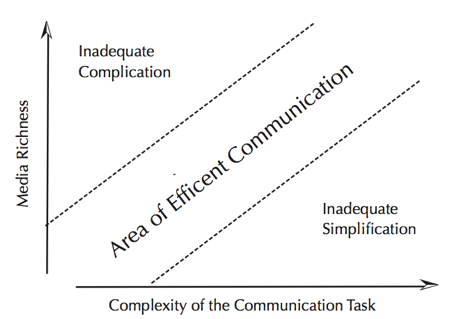
\includegraphics[height=2in]{images/media-richness-model.png}
	\caption{The Media Richness Model \citep{Rice1992}}
\label{fig:images_media_richness_model}
\end{figure}

Due to the task complexity a \textbf{physical face-to-face meeting} with representatives of all stakeholders involved might be a good fit, but arranging such a meeting (same time, same place) with multiple parties, that are globally dispersed, is either economically not feasible or takes a lot of time. But the more time passes for investigating the crime, the more difficult it will become to identify the fraudsters and take legal actions against them. Acting immediately can therefore reduce the risk of losing the money completely. \\

As of these conditions a \textbf{computer-supported collaborative work} (CSCW) system might be an alternative to \textit{cooperate} on an incident of E-commerce fraud (same time, different place). CSCW systems can be categorized by their support for the mode of group interaction as done in the 3C model: \@

\begin{itemize}
    \item\textbf{communication:} two-way exchange of information between different parties
    \item\textbf{coordination:} management of shared resources such as meeting rooms
    \item\textbf{collaboration:} members of a group work together in a shared environment to reach a goal
\end{itemize}

Based on the level of support for one of these functionalities the various systems can be classified and described (see Figure~\ref{fig:images_3C_model}) \citep{Koch2008}: \@

\begin{figure}[H]
	\centering
		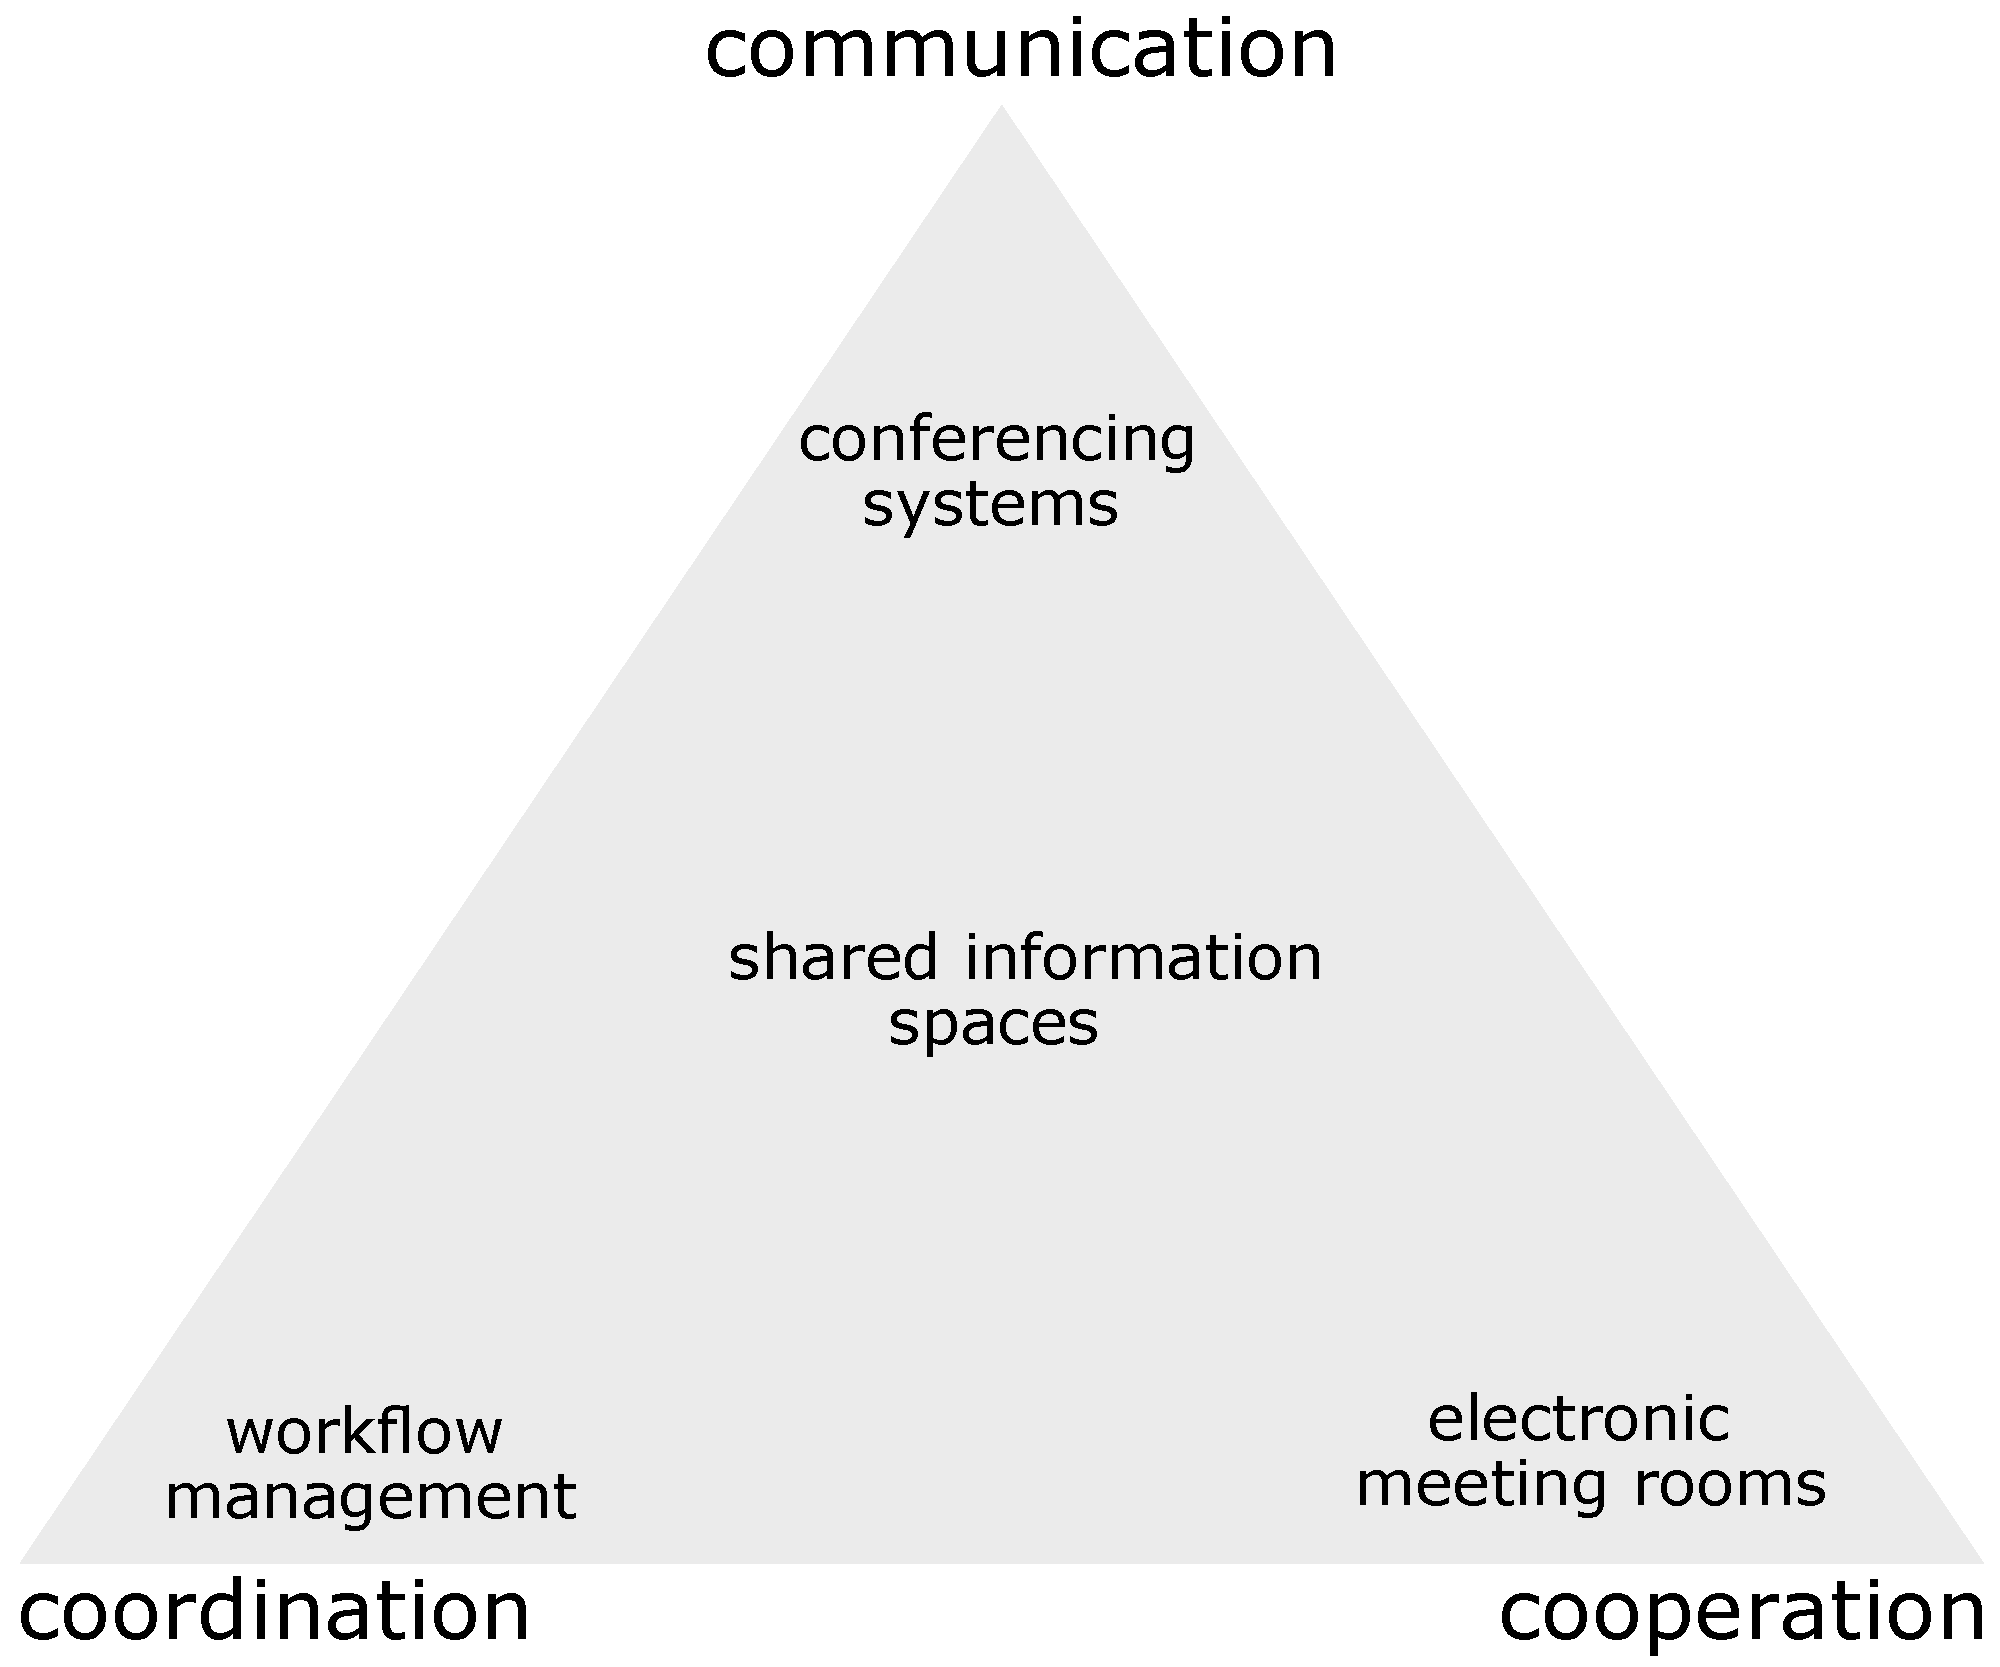
\includegraphics[height=2.5in]{images/3C-model.pdf}
	\caption{The 3C Model \citep{Koch2008}}
\label{fig:images_3C_model}
\end{figure}

A good candidate for such a collaborative system \textit{could} be a \textbf{shared information space}; aka team rooms, cloud storage services or document management systems, that allow participating parties to access information at any place, any time and to share information between each other --- usually with a build in versioning support for artefacts and a workflow component. \\

However, as some of the required information might be confidential or business-critical to one of the involved parties, a \textbf{centralized system} (e.g.\ a service in the cloud) can \textbf{\underline{not}} be used in the scenario described here. Another key characteristic of the investigation of an E-commerce fraud is the fact that it involves information sharing from many different organizations. These different aspects have to be combined into a \textbf{shared information space} in a meaningful way to be able to achieve the common group goal on time. Combining information from different stakeholders will face issues due to \textbf{different wordings and data formats} of the information, \textbf{competing incentives} of the stakeholders to participate on information sharing as well as possible \textbf{sharing restrictions}, that prevent making the information available to a larger audience. \\

\textbf{Decentralized information sharing architectures}, that utilizes \textbf{peer-to-peer communication technologies}, are either restricted to a commonly agreed set of data entities and relations (based on an ontology) between all parties involved or are lacking richer semantics for sharing and integrating content between the stakeholders. \textbf{Semantic Web technologies} can help lower the barrier to integrate information from various sources into a shared information space, and the advantages of peer-to-peer communication and Semantic Web technologies for information sharing in distributed, inter-organizational settings have been shown in \citep{Staab2006}. \\

Still these studies concentrate on making information from different parties searchable and accessible in a distributed, shared information space, in which data can be accessed and queried at any time from any participating party. They are not solving the problem of working collaboratively on a common goal in an ad-hoc, loosely-coupled virtual team of disperse organizations by making certain (sometimes sensitive) information available in a shared environment. \\

Therefore, the \textbf{research question} for this Master thesis can be summarized as follows: \@

\begin{quotation}
  \textit{In how far can a computer supported collaborative work system based on peer-to-peer communication technologies and shared ontologies improve the efficiency and effectivity of E-commerce fraud investigations within an inter-institutional team?}
\end{quotation}

% section problem definition (end)


% sub chapter outline of thesis
%!TEX root = ../MasterThesis.tex

\section{Master Thesis Outline}
\label{sec:thesis_outline}

Before starting with the investigation of \gls{E-commerce} fraud incidents and their possible examinations, the thesis starts with a description of related works in Chapter~\ref{cha:related_works}, that have been looked into during the course of this Master thesis and have had an influence on it. \\

In the next part, Context Analysis in Chapter~\ref{cha:context_analysis}, the thesis discusses the \gls{E-commerce} scenario in detail. It starts with a description of the \gls{E-commerce} shopping process, looks into the stakeholders involved as well as shows possible kinds of \gls{E-commerce} fraud incidents and how they are handled today. Based on these findings this chapter closes with a presentation of the specific scenario, that has been selected for further examination within this Master thesis. \\

After this initial scope setup the thesis briefly outlines the theoretical foundations required for the understanding of the concepts in the solution space in Chapter~\ref{cha:theoretical_foundations}. This section starts with a short overview of the relevant facets of computer-supported collaborative work systems (\gls{CSCW}), shows the essential specifications of the Semantic Web, and ends up with an introduction to the peer-to-peer (\gls{P2P}) communication techniques and protocols. \\

In the main parts of this thesis (Chapter~\ref{cha:system_concept} and Chapter~\ref{cha:system_design}) the concept and design for a collaborative system, that supports the investigation of \gls{E-commerce} fraud incidents, is discussed. These chapters will lay out and analyze the possibilities for designing and using such a collaborative system. The objective is to come up with an approach at the end of the discussions, that might be the best fit for the problem described in the scenario at the beginning. \\

To conclude the thesis also sum up the findings and give an outlook for future work on this topic.

% section thesis outline (end)


% chapter introduction (end)


	% The counter for tables and figures are set back in order to start a new numeration per chapter
\setcounter{table}{1}
\setcounter{figure}{1}
	% Inclusion of the third chapter
	%!TEX root = ../MasterThesis.tex

\chapter{Related Works}
\label{cha:related_works}

Gayatri R. Ankhule et al. give an overview of \gls{E-commerce} and specify the different types of it. In addition to that the authors also show the positive and negative impact of the current implementation of \gls{E-commerce} for organizations, individuals and society in general. After demonstrating the advantages of it (and the reasons for the growing success) they assert that the safest way to checkout an order on a Web shop is by using a credit card, because in the case of fraud attempts on a credit card consumers can rely on regulations and protection laws in place to rollback malicious transactions. At the end of the paper they conclude that a successful \gls{E-commerce} shop is not just a technical problem, but affects the whole business operation \citep{ankhule2015overview}. \\

The paper from Sobko discusses what non-cash transactions are and shows ways how fraudsters try cheat the system. It starts with a classification of non-cash payments including credit and debit cards that are handed out by financial institutions to individuals for doing commerce. The authors also note the ways to trick an individual with the objective to get access to credit card information such as phishing and skimming. They notice that once a transaction has been successfully executed with a stolen credit card the information about it will be sold on the black market to other fraudsters, who will then use the same credit card to make larger purchases. Further on the paper discusses the impact of fraudulent transactions on the merchants and credit card owners, as well as discusses technological advances and legislations that have been developed to protect against non-cash frauds \citep{sobko2014fraud}. \\

The study of Pritikana Sen et al. starts with an introduction to the subject of \gls{E-commerce} and iterate on the classification of it. It states the benefits of \gls{E-commerce} (e.g.\ the global reach of Web shops) as well as its limitations. Here it mentioned explicitly the security of the system and the communication protocols used. The paper lists the relevant stakeholders of an \gls{E-commerce} transaction and describes the credit card payment process. It concludes with an analysis of the security features of a Web shop and shows that those are not limited to technical aspects alone, but always include the consumer and his behavior on the Internet \citep{sen2015study}. \\

The research of Priya J. Rana et al. shows possible frauds in \gls{E-commerce} and how they can be detected with current fraud prevention systems. The show different implementations of fraud detection algorithms that range from simple rule-based filtering to score-based solution using fuzzy logic. They conclude that general systems in use can cover up to 80\% of fraudulent transactions at manageable efforts and costs. More coverage can be achieved by combining existing solutions with information of the card owners profile, which introduces credit card usages patterns into the analysis. Still this solution is very expensive to implement and operate \citep{rana2015survey}. \\

The paper from Carvalho et al. looks into the financial crime investigation process by using banking frauds as example. It shows that the investigation is a complex task that needs further collaboration between experts. Still just sharing the information will not be enough as a common understanding of the different aspects and terms is required. Therefore they state that finding a common language to exchange information is very important for the success of the investigation. Based on this finding the paper also develops an ontology to describe the domain of banking fraud investigation. It elaborates on the objects and their relations in detail and shows that reusing concepts and terms from existing vocabularies can be helpful when designing an own ontology. The paper concludes that semantic technologies can have a positive impact on the crime investigation as they are providing basic reasoning capabilities on the data sets as well as merging information from different sources. These features will allow a crime investigator from a law enforcement agency to inspect and analyze more complex information. Finally the paper considers semantic technology to be very important in future cybercrime inspection \citep{carvalhoapplying}. \\

The seminal paper ``Linked data-the story so far'' explains the fundamental concepts, approaches and technologies to share data on the Web. It shows how a \gls{RDF} data set should be used to publish structured data on the Web and provide rules how these resources should be described ideally. Additionally it discusses the open and commonly used vocabularies available on the Web, as well as shows ways how to link together different resources on the Web. After describing different kinds of applications that are possible with the technologies mentioned it gives an outlook of future research, which also contains the aspects of schema mapping and data fusion. Another challenge in the area of Linked data are possible privacy violations due to combining information from different sources. As conclusion the paper sees the Linked data approach as intermediate step to a Semantic Web, because it also follows established Web standards such as \gls{RDF}, \gls{RDFS} and \gls{SPARQL}, but it uses a more pragmatic approach by getting rid of all the complexities involved when having to create, maintain and use large ontologies in \gls{OWL} \citep{bizer2009linked}. \\

- ``Linked data-as-a-service: the semantic web redeployed'' \citep{rietveld2015linked}

- ``Goodrelations: An ontology for describing products and services offers on the web'' \citep{hepp2008goodrelations} \\
- ``Schema.org: Evolution of structured data on the web'' \citep{guha2016schema} \\
- ``Leveraging WebRTC for P2P content distribution in web browsers'' \citep{vogt2013leveraging} \\
- ``Content-centric user networks: WebRTC as a path to name-based publishing'' \citep{vogt2013content}

% chapter related works (end)


	% The counter for tables and figures are set back in order to start a new numeration per chapter
\setcounter{table}{1}
\setcounter{figure}{1}
	% Inclusion of the second chapter
	%!TEX root = ../MasterThesis.tex

\chapter{Context Analysis} % (fold)
\label{cha:context_analysis}

This chapter will look into the scenario of e-commerce fraud investigation in detail.
It will start with an in-depth scenario description followed by an analysis of all involved stakeholders.
It will further describe the kind of information each stakeholder has in her local context and her objectives to take
part on the information sharing and collaboration initiative. The chapter ends with a description of the scope
this Master thesis will focus on.

% sub chapter scenario description
%!TEX root = ../MasterThesis.tex

\section{An overview of \gls{E-commerce}}
\label{sec:e_commerce_scenario}

\gls{E-commerce} as a term relates to the trading of products or services utilizing a computer network such as the Internet. It is usually categorized into the following four different subfields \citep{sen2015study}:\@

\begin{enumerate}
  \item \textbf{Business-To-Business (\gls{B2B})}: refers to electronic trading between companies with the objective to improve their supply chain processes
  \item \textbf{Business-To-Consumer (\gls{B2C})}: refers to electronic trading between a company and its consumers (most publicly known example for it is Amazon \citep{Amazon.com})
  \item \textbf{Consumer-To-Consumer (\gls{C2C})}: refers to electronic trading between consumers (most publicly known example for that is eBay \citep{eBayInc})
  \item \textbf{Consumer-To-Business (\gls{C2B})}: refers to electronic trading between consumers and businesses (most publicly known example for this is TaskRabbit \citep{TaskRabbit})
\end{enumerate}

This Master thesis will \textbf{\underline{solely}} focus on the \gls{B2C} aspect of \gls{E-commerce}. In that case a consumer is using an \gls{E-commerce} shop of a merchant on the Internet to order products or services online. The merchant is offering a catalog of available products or services on the Web, that is available and accessible by the general public and usually has a nation-wide if not global reach. The merchant can either run the \gls{E-commerce} shop software on their own servers (on-premise) or can outsource this additional sales channel to a 3$^{rd}$ party hosting company or cloud service provider (\gls{CSP}). Also the \gls{E-commerce} shop software itself can be either developed by the merchant in-house or acquired as a boxed product from an Independent Software Vendor (\gls{ISV}) on the market. For business accounting purposes the merchant also runs a bank account with the acquirer (see Figure~\ref{fig:images_ecommerce_scenario}). \\

When placing an order with the merchant online, the consumer is usually using a credit card for finalizing the transaction. This credit card has originally been handed out by the issuing bank to the consumer. Additionally, in some online shops it is mandatory for the consumer to create an user account with them, while in others it is not. The former is the preferred way when consumers are repetitively buying from that merchant, whereas the latter might be used for one-time or irregular shopping trips online. To be able to connect to the Internet the consumer also relies on a service of an Internet Service Provider (\gls{ISP}). The whole initial setup for participating on \gls{E-commerce} activities is found in Figure~\ref{fig:images_ecommerce_scenario}.\@

\begin{figure}[H]
	\centering
		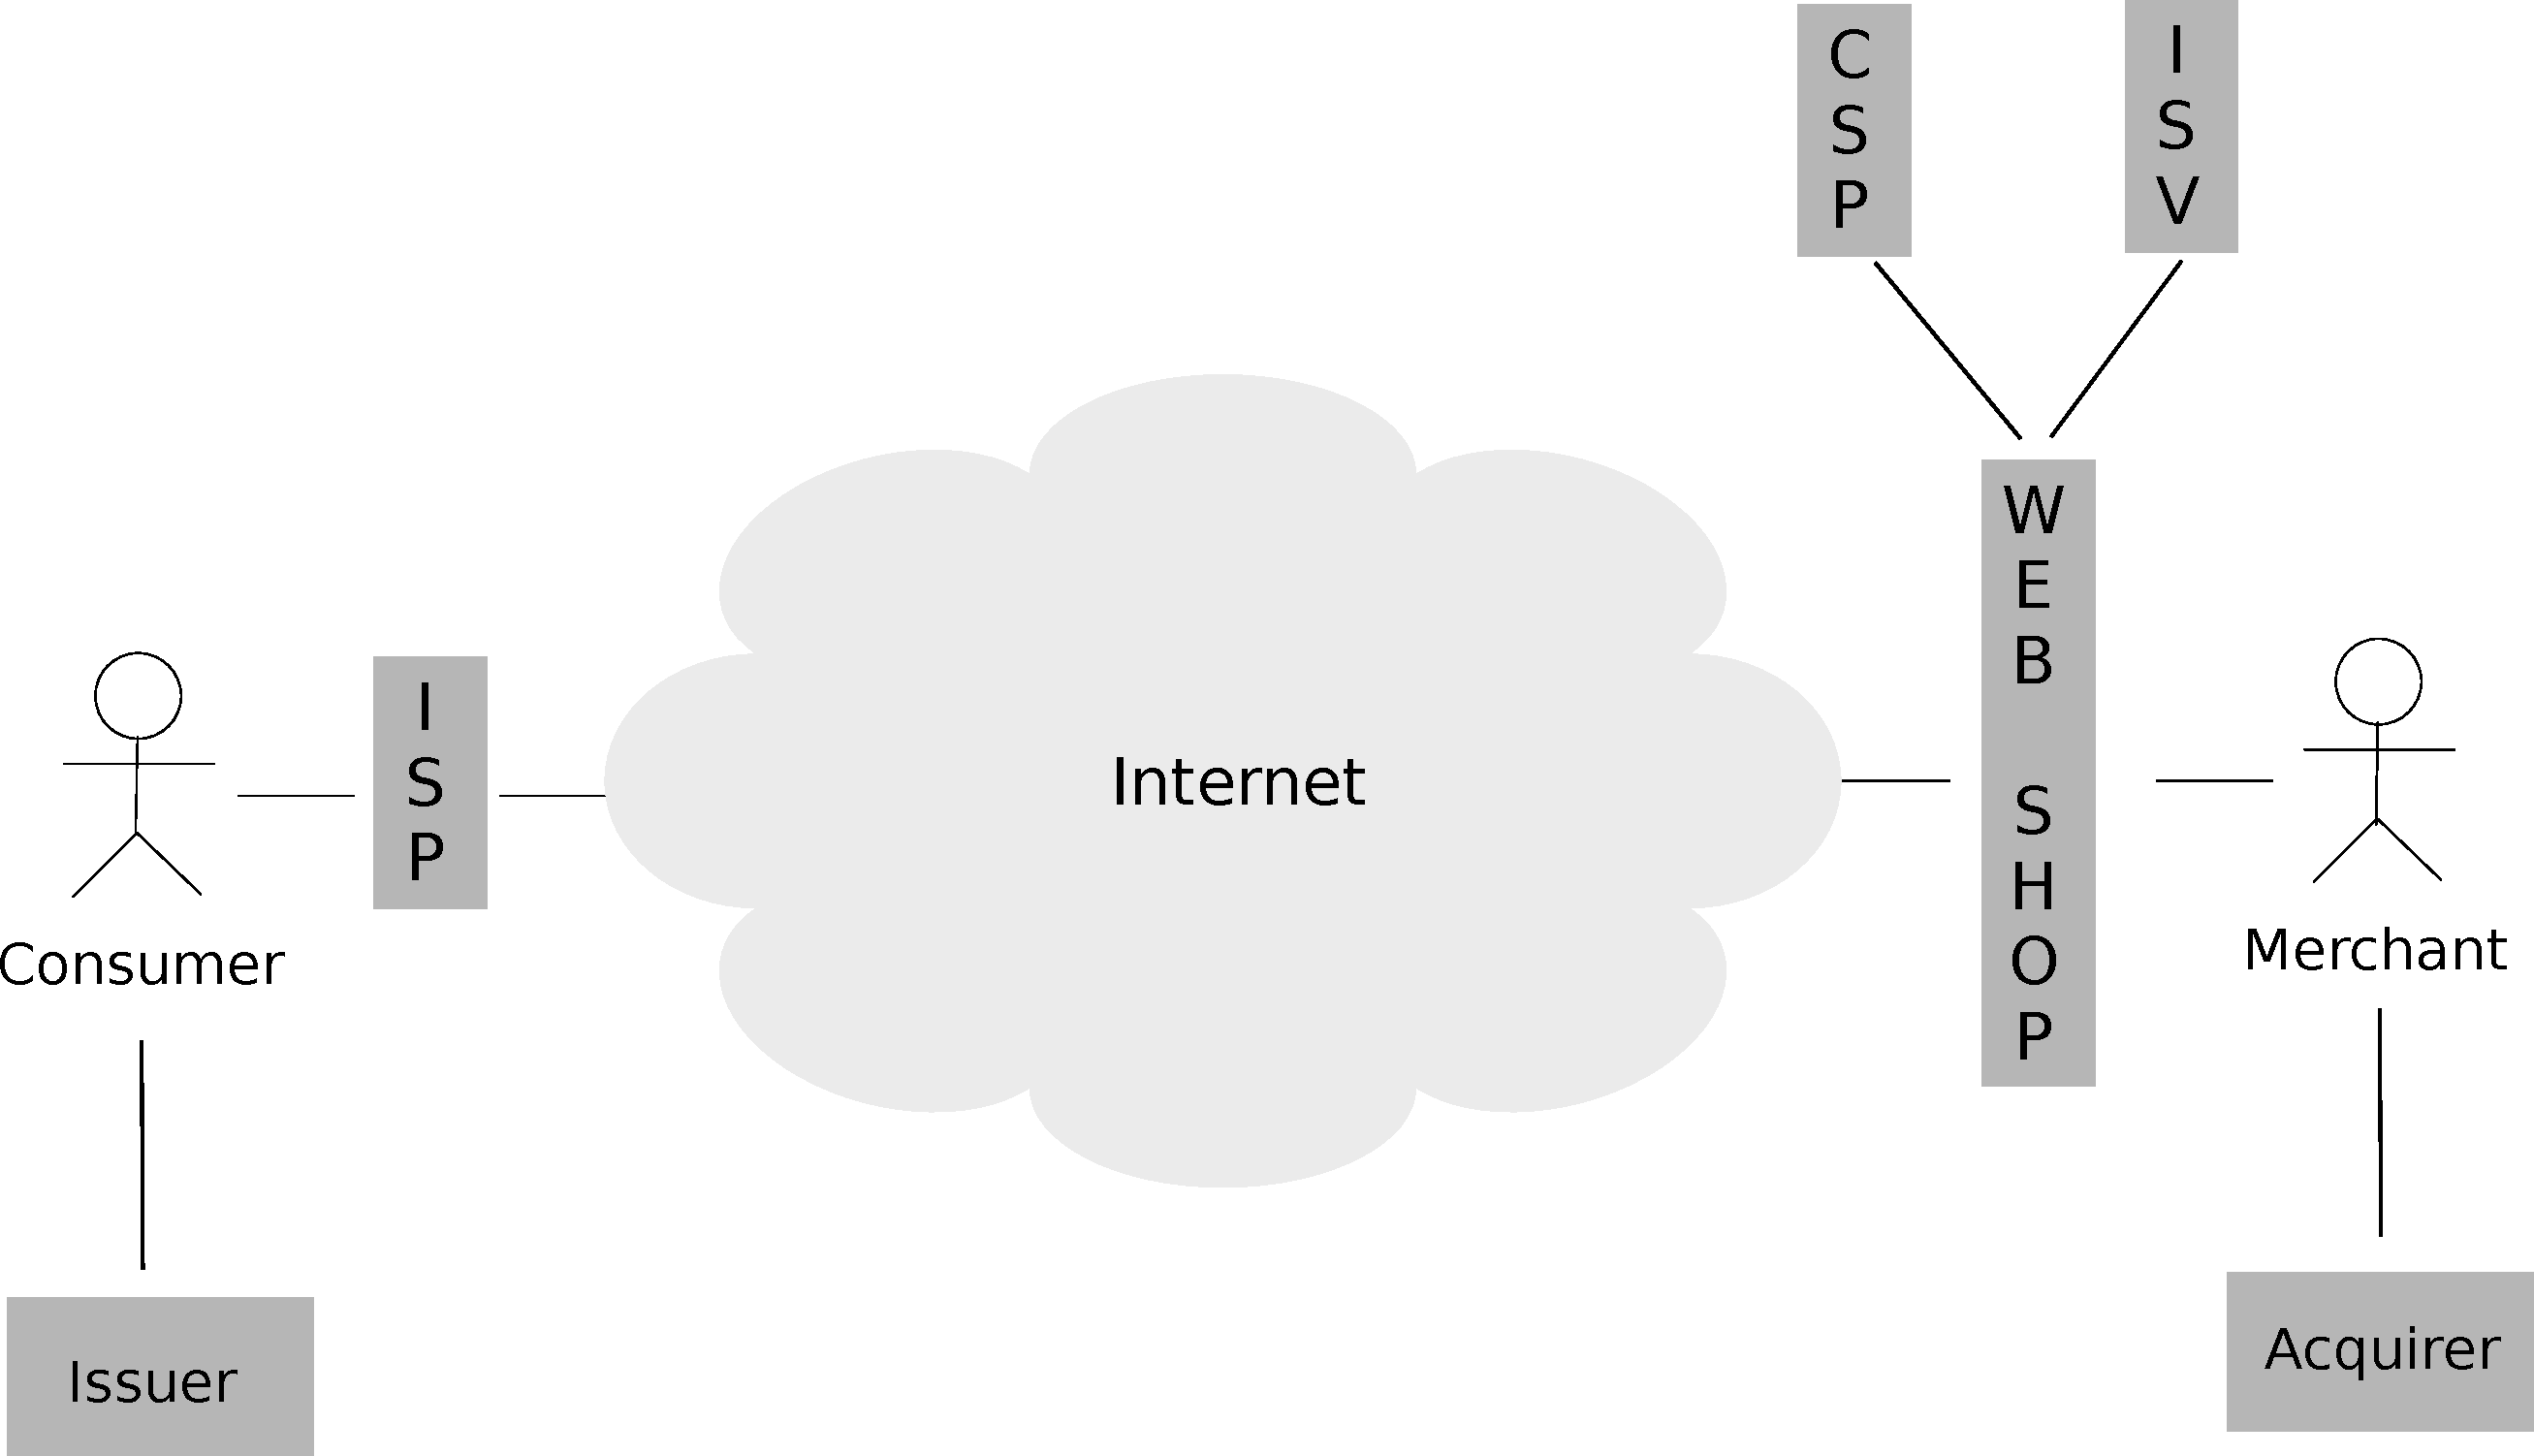
\includegraphics[width=0.8\columnwidth]{images/e-commerce-scenario.pdf}
	\caption{\gls{E-commerce} Fundamentals}
\label{fig:images_ecommerce_scenario}
\end{figure}

When the consumer places the order online, the merchant receives at least a list of products or services from the current shopping cart of the consumer, the identification of the consumer as well as the delivery address to ship the physical items to. If the transaction is going to be finalized with a credit card, the consumer will have to provide additional information like their billing address and credit card information (including the id, the expiry date and the security number of the card). \\

The merchants usually doe not validate the credit card information on their own. For that purpose they are relying on another 3$^{rd}$ party service offered on the Internet by the Payment Service Provider (\gls{PSP}). These providers are either validating the credit card information themselves based on an user profile the consumer has with the \gls{PSP} (e.g.\ a globally available Web service such as PayPal), or are connecting to the issuing bank of the credit card for doing so. For initiating this validation process the merchant is handing over the billing information to the \gls{PSP} incl.\ the credit card information given by the consumer. \\

Either the \gls{PSP} or the issuing bank is validating the correctness of these information with criterias like: \@

\begin{itemize}
    \item is the billing address matching the current consumers' postal address on file?
    \item is the stated credit card information correct?
    \item is the credit card still valid?
    \item is the credit card not marked as being blocked in the internal databases?
\end{itemize}

The merchant will receive the status of the authorization as well as an unique payment token in return. If the authorization was done successfully, the merchant will collect the items and send out a shipping request to one of the available Logistic Service Providers (\gls{LSP}), that are capable to handle the delivery of the order. They will pickup the items at the merchant's facility and ship them to the delivery address stated by the consumer. Usually in parallel the merchant is informing their bank about the order, amount due as well as the payment token received from the \gls{PSP}. The acquirer is in charge to withdrawal the amount of the order from the consumer's bank account either via the \gls{PSP} or directly from the issuing bank, depending on who of them has authorized the initial payment request (a process called clearing) \citep{VisaPayment2014}. The sequence of activities within an \gls{E-commerce} checkout process is visualized in Figure~\ref{fig:images_ecommerce_checkout_process}.\@

\begin{figure}[H]
	\centering
		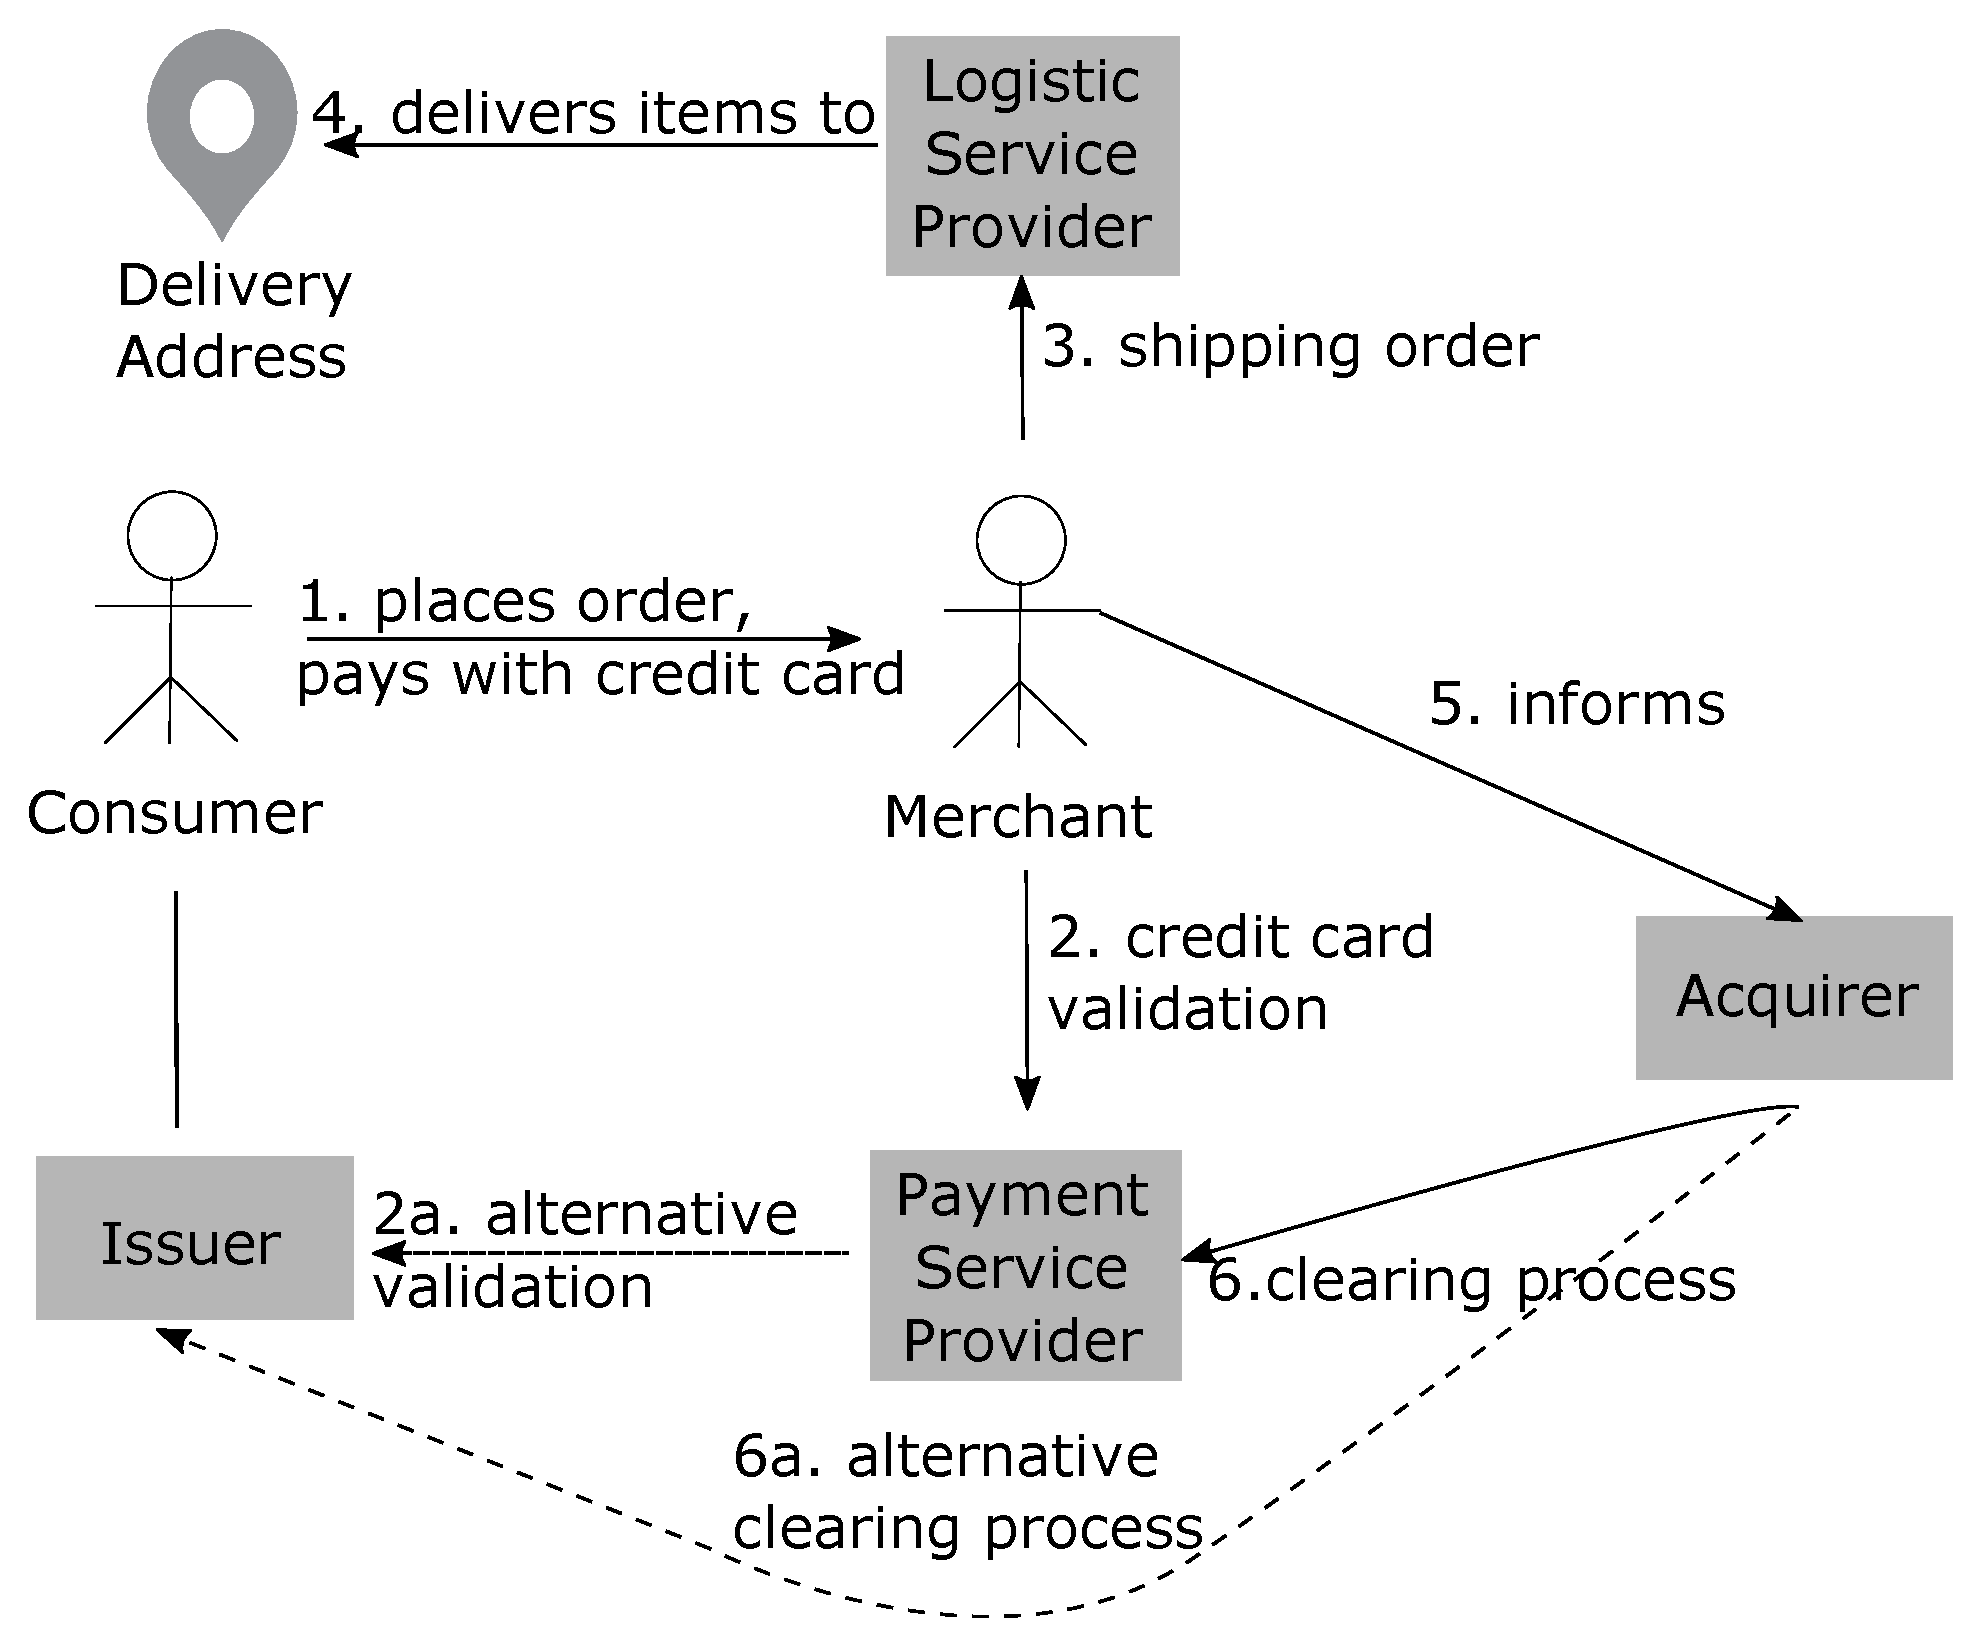
\includegraphics[width=0.8\columnwidth]{images/e-commerce-checkout-process.pdf}
	\caption{\gls{E-commerce} Checkout Process in detail}
\label{fig:images_ecommerce_checkout_process}
\end{figure}

% section scenario description (end)


% sub chapter stakeholder analysis
%!TEX root = ../MasterThesis.tex

\section{Stakeholders}
\label{sec:stakeholder_analysis}

The following section looks at each stakeholder involved in the E-commerce scenario in detail, lists the kind of information they own or provide to others as well as describes the role of each stakeholder in the E-commerce fraud investigation process (if any).

\subsection{Consumer}
\label{subsec:stakeholder_consumer}

The consumer is the initiator of an E-commerce transaction. She is using the shop of a merchant on the Internet to order products or services. For doing so she has to know the \gls{URL} of the Web shop, has to be connected to the Internet via the \gls{ISP} and has to use a standard software called a Web browser on her computer. For the duration of her online browsing session she also owns an unique \gls{IP} address handed out from the \gls{ISP}.\\

She might have had a long-term business relationship with the merchant and already owns an user account on the Web shop. On the other hand she might be just interested into a one-time shopping trip and might want to order the items without creating an account first --- sometimes also called ``anonymous checkout'' in the E-commerce shops. \\

The consumer is also having a bank account and at least owns a debit card with the issuing bank to get access to the money on that account. In addition to that she can also hold multipe credit cards. A credit card can be issued by the same bank or can be provided by another financial service (e.g. American Express). In any case the organisation that has handed out the credit card to the consumer is called the issuer. \\

If she is going to order items in a Web shop, she will usually browse the product and service offerings of the merchant first and put the items of interest into the shopping cart. When finalizing the transaction she has to state the following information to the merchant:\@

\begin{itemize}
		\item personal information incl.\ given name, family name and date of birth
		\item the address the items should be shipped to
		\item payment information incl.\ type of payment and billing address (if different to shipping address)
\end{itemize}

If she is going to end the transaction with a payment of type credit card she will also have to provide specific information of the card, that should be used for the payment:\@

\begin{itemize}
		\item the owner of the credit card (if it is not belonging to herself)
		\item the unique credit card number
		\item the expiry date of the credit card (in format MM/YY)
		\item the security code of the credit card
\end{itemize}

The consumer is having a special role in the whole scenario. As the online merchant has to deal with the consumer without any face-to-face or real-world interaction, the consumer is also the least thrustworthy party from the point of view of the merchant. As the Section~\ref{sec:scenario_fraud} will show, the consumer is the main object of question in the case of an E-commerce fraud incident. For the investigation of it the consumer is usually not taking any active part.

% subsection stakeholder consumer

\subsection{Merchant}
\label{subsec:stakeholder_merchant}

The merchant offers products and services on the Internet to the general public. She might use the Internet as an additional sales channel, or rely on it solely for making any business. To provide access to the Web shop the merchant has to register a domain name and an \gls{URL} with a local domain name registry. This specific \gls{URL} refers to a fixed public \gls{IP} address, that the server that runs the Web shop software uses. Normally the merchant does not operate the servers herself, but rely on a service offering from a hosting or cloud service provider for that. Also the Web shop software itself is usually not provided by the merchant, but bought from an \gls{ISV} on the market. In any case the merchant has special responsibilities in the Web shop, because she has to take care to configure the products, prices, promotions, payment and shipment services available. In addition products can be categorized by her into departments and sub-departments for easier navigating and searching the offerings in the Web shop by the consumer. \\

The merchant can decide whether she restricts ordering of products to registered users only, or allows anonymous users too. The main benefit of the former is the possibility to analyse the shopping behaviour of individual consumers, whereas the latter will open the business for a wider range of consumers as it includes also those, that do not want to register with any existing online shop. Nevertheless, any consumer activity on the online shop is tracked in the analytic databases of the merchant. This includes not only the items, that have been placed into the shopping cart, but also any product that has been looked at by the consumer during a shopping session. Even if these detailed analytic capabilities are actually synonymous for their usage in target-related advertising, they can also help to decide whether a consumer behaves normally or not. \\

Any business transaction that the consumer makes with the merchant is stored in the merchant's databases. A transaction information contains, but is not limited to:\@

\begin{itemize}
		\item the personal information of the consumer
		\item the address the items will be shipped to
		\item a collection of products with quantities and prices
		\item the total amount of the order considering promotions, taxes and fees
		\item the selected payment information
\end{itemize}

If the consumer pays with credit card, the merchant will not handle the payment herself, but relate this activity to a Payment Service Provider. To initiate the credit card authorization request, the merchant is sending the following information to the Web service endpoint of the \gls{PSP}: \@

\begin{itemize}
    \item consumer's billing address
    \item given credit card id, expiry date and security number
    \item identification of the merchant
    \item final amount of the current transaction
\end{itemize}

In return of the payment authorization the merchant will receive and store these  payment-related information for the transaction:\@

\begin{itemize}
		\item the type of credit card used (e.g. Visa, MasterCard, American Express, \ldots)
		\item the name of the credit card owner
		\item the payment token received by the \gls{PSP}
		\item the timestamp and result code of the authorization
		\item the authority who approved the payment (if the merchant works with multiple Payment Service Providers)
\end{itemize}

As a merchant will collect a lot of personal and payment-related information over time, she is also one of the major sources of possible data leaks in this scenario. Due to this circumstance the Payment Card Initiative, a group of banks, issuers and \gls{PSP}s, provides rules and guidelines (aka PCI/DSS standards) for securely handling these kinds of information in an IT system \citep{virtue2009payment}. \\

A merchant is one of the main actors in the fraud investigation process. She is highly interested in figuring out whether the consumer's transaction is valid or not. That is due to the fact, that in case of an E-commerce fraud incident the merchant will mostly have to cover the costs (see Section~\ref{sec:scenario_fraud}). Also the online merchant's reputation will suffer, if private information from her databases get leacked. If a merchant falls victim to a fraud incident multiple times, the economic damages can finally result in a bankruptcy of the merchant.

% subsection stakeholder merchant

\subsection{Payment Service Provider}
\label{subsec:stakeholder_psp}

The Payment Service Provider is offering payment-related services to online merchants. To be able to do this the \gls{PSP} provides a common Web interface, that the merchant has to communicate with for sending payment authorization requests (see above). The \gls{PSP} might be able to authorize the payment request on her own, or have to route the request to the corresponding issuer of the credit card in question. For the former procedure the \gls{PSP} has to run an own database of registered users with their credit card information (e.g.\ a Web service such as PayPal). For checking the credit card and authorizing the payment the merchant is sending the following information from the transaction:\@

\begin{itemize}
		\item credit card owner incl.\ billing address given
		\item credit card number
		\item credit card expiry date
		\item credit card security code
		\item identification of the merchant
		\item total amount of the current transaction
\end{itemize}

The \gls{PSP} has to securely process these information and return the result of the validation to the merchant. The result message also contains an unique payment token, that the merchant can refer to later to initiate the clearing process. As of this the \gls{PSP} has to persist the credit card and transaction-related information in her own backend databases. Following industry standards, she should do so according to the PCI/DSS guidelines mentioned in the previous section. \\

The level of activity in the E-commerce fraud investigation process depends on whether the \gls{PSP} authorizes the payment herself, or only acts as routing service between the merchant and the original credit card issuer. In the former case the \gls{PSP} is more actively involved. In that situation she also holds more of the valuable information to analyze the incident. In the latter case she will still be required to connect the payment-related request information from the merchant with the corresponding authorization result coming from the issuer.\\

If the \gls{PSP} holds sensitive information in her own databases, she will also be a source of possible data leaks. In that situation she has to put the same precautions in place as an issuing bank will have to do (see next section).

% subsection stakeholder psp

\subsection{Issuing Bank}
\label{subsec:stakeholder_issuer}

The issuer is one of the parties in the scenario that knows the owner of the credit card in person. Each individual has to register personally with the issuer to get access to a credit card. This registration process includes providing the following information: \@

\begin{itemize}
		\item personal information such as given name, family name and date of birth
		\item the currently registered home address
		\item the bank account that should be used to settle credit card balances
\end{itemize}

Even if the two parties do not really meet each other personally, an individual will still have to identify with a valid id card and bank account to receive and activate a new credit card. Beside being the single source of truth about the original credit card owner, the issuer of the card also collects and stores all  usages of it. The issuer therefore can provide individual credit card usage patterns, that are not just limited to the online shopping scenario --- something a Payment Service Provider can deliver too; but also include transactions the card owner does in the real-world. Needless to say that these are valuable information for the E-commerce fraud investigation. \\

Still the issuer does not know the details of the transactions, that have been made with the credit card yet. As shown in the Section~\ref{subsec:stakeholder_psp} the issuer will just receive an identifier of the merchant, in whose shop the credit card has been used. Based on public available information from a commercial register about the merchant, the issuer could at least come up with the retail branch the merchant operates in. \\

Being the single source of truth about all issued credit cards, their owners and usage patterns makes the issuer another high-risk participant for possible data leaks. She should as well follow the guidelines from the PCI/DSS standards, should incorporate security standards for her IT systems and processes as well as monitor her backend systems actively with an intrusion detection mechanism.

% subsection stakeholer issuer

\subsection{Acquiring Bank}
\label{subsec:stakeholder_acquirer}

The acquirer holds the bank account of the merchant and is responsible for withdrawing the outstanding amounts of transactions from the accounts of the consumers, or more precisely requesting it from the issuing bank of each consumer. As of this the acquiring bank is usually not processing any credit card related information from consumers, but refer to the payment tokens that have been given by the \gls{PSP} or issuer during the authorization process. \\

Still as a financial institute the acquirer (like the issuer) has to comply with the rules and guidelines of the PCI/DSS and other industry standards to make sure, that her bank accounts and the transaction processing are safe and secure. The detailed analysis of these techniques and procedures as well as possible banking fraud incidents are out of scope of this Master thesis though.

% subsection stakeholder acquirer

\subsection{Logistic Service Provider}
\label{subsec:stakeholder_lsp}

The Logistic Service Provider has two important roles in the E-commerce scenario. First, she has access to and control over the items of the merchant for the duration of the transport between the merchant's facility and the consumer's shipping address. And second, she holds the information to whom she has handed over the items at the final destination. Although the \gls{LSP} has nothing to do with any payment-related activities, she is still critical as she will be the last chance for the merchant to stop the delivery of the items (in case a fraud has been detected after initiating of the shipment), or provide information about the person that has received the items at the shipping address --- especially so on high-priced goods, that usually require the recipient to show her personal id card and place a signature on the delivery receipt. \\

For initiating the shipment procedure the merchant is ordering a certain transport service from the \gls{LSP} and hand over the following information:\@

\begin{itemize}
	\item name of the receiver
	\item delivery address given by the consumer
	\item list of items to be shipped
	\item optionally: value of the items if an insurance policy is taken
\end{itemize}

The \gls{LSP} at the other hand returns an unique tracking id for the shipment. It can be used by the merchant and the consumer to check the status of the shipment online. \\

As the \gls{LSP} does not have to deal with the payment-related activities in the E-commerce scenario, she is also not actively involved in the fraud investigation. Still she is of help, if an incident is found as she can stop the delivery or provide useful information about the recipient.

% subsection stakeholder lsp

\subsection{Cloud Service Provider}
\label{subsec:stakeholder_csp}

The Cloud Service Provider offers IT services to its customers. These IT services include hardware and software assets, that (in the E-commerce scenario) a merchant can order to run her Web shop on the Internet. Part of the service level agreement between the merchant and the \gls{CSP} is a detailed listing of the responsibilities of both parties (who has to take care of what). In most cases the merchant is outsourcing the complete operation of the hardware and software for the Web shop to the \gls{CSP}; so the \gls{CSP} will be responsible for making sure that the Web shop is accessible and secure. The \gls{CSP} is also constantly monitoring the incoming connections to each public Internet server under her control and can provide information, whether a Web shop of one of the merchants has been compromised or not.

% subsection stakeholder csp

\subsection{Independent Software Vendor}
\label{subsec:stakeholder_isv}

The \gls{ISV} designs, implements and sells the Web shop software. She has detailed knowledge about the software components and libraries used within the Web shop and checks them regularly for security breaches or vulnerabilities. She also has to verify the software code implemented on her own for vulnerabilities, and has to make sure that the implementation follows industry standards (e.g. PCI/DSS for handling person and payment-related information). Therefore she can best assert these quality criterias of the Web shop software if needed.

% subsection stakeholder isv

\subsection{Internet Service Provider}
\label{subsec:stakeholder_isp}

The \gls{ISP} provides a service to the consumer, so that she is able to connect to and use the Internet. Each Web request the consumer is doing on her system is routed to the public Internet via the infrastructure of the \gls{ISP}. Due to existing regulations and laws the \gls{ISP} has to store the log files of any Internet session of its customers for a certain amount of time. Especially, these log files can be helpful to decide whether a consumer was visiting pages in the dark-side of the Web, or if she falls victim to some phishing attacks (explained later in Section~\ref{sec:scenario_fraud}).

% subsection stakeholder isp

% section stakeholder analysis


% sub chapter stakeholder objectives
%!TEX root = ../MasterThesis.tex

\section{Stakeholder Objectives}
\label{sec:stakeholder_objectives}

% section stakeholder_objectives (end)


% sub chapter scope of thesis
%!TEX root = ../MasterThesis.tex

\section{Scope of this Master Thesis}
\label{sec:scope_thesis}

As laid out in the previous section, the most interesting E-commerce fraud scenario is the one, in which a fraudster uses a leaked credit card information to order products or services from various merchants on the Internet. This is currently most likely to be successful, because there is a lack of information on the side of the merchant as well as the \gls{PSP} or issuer. Each of the affected merchants just noticed the single transaction that takes place on her own Web shop, without knowing about the other attempts the fraudster do on other Web shops. The \gls{PSP} and issuer will notice the active use of the credit card on different Web shops though, but do not have any information about the transaction details. Therefore they could not correlate these information to check for suspicious activities. \\

Based on the current credit card usage patterns of the fraudsters, whose will use a leaked credit card information in commonly used Web shops, which deal with electronics, entertainment or travel-related products and services, it is more likely that these fraudulent transactions will not be recognized on time by the existing fraud prevention mechanisms in place today. \\

A simple approach to solve this issue would be to just share more information of the ongoing transaction between the merchants, the \gls{PSP}s and the issuers. This might be subject to fail though, because each party has to follow the restrictions and regulations for sharing personal-related information. Additionally adapting and harmonizing the communication interfaces between the Web shops from various online merchants and the Web interfaces of different \gls{PSP}s and issuers are an enormous undertaking and will likely not succeed due to different notions of the communication patterns and data structures exchanged between all relevant participants. \\

This shows the scenario this Master thesis will look into in detail and try to solve the most important question: \textit{is this really a fraudulent transaction?} \\

Looking into the stakeholders, that can provide useful information to decide on it, one will come up with:\@

\begin{enumerate}
    \item \textbf{merchant}, who can provide additional information of each E-commerce transaction in question
    \item \textbf{\gls{PSP}/issuer}, whose offer information about the credit card usage pattern and the original credit card owner
    \item \textbf{\gls{LSP}}, who can offer information about whether the order has already been shipped or not, and in the former case to whom it has been handed over
    \item \textbf{\gls{ISP}}, who can on request give hints whether a consumer has fallen victim to a phishing attack based on her Internet access logs
\end{enumerate}

% section scope_thesis (end)


% chapter context analysis (end)


	% The counter for tables and figures are set back in order to start a new numeration per chapter
\setcounter{table}{1}
\setcounter{figure}{1}
	% Inclusion of the third chapter
	%!TEX root = ../MasterThesis.tex

\chapter{Theoretical Foundations} % (fold)
\label{cha:theoretical_foundations}

This chapter will lay out the theoretical foundations for the to-be-designed collaborative system. It will start with an investigation of the \gls{CSCW} system theory followed by a detailed examination of the Semantic Web standards such as \gls{RDF}, \gls{OWL} and \gls{SPARQL}. Last but not least the chapter will look into the core concepts of \gls{P2P} communication technologies and protocols such as \gls{XMPP} and \gls{WebRTC}.

% sub chapter computer supported collaborative work systems
%!TEX root = ../MasterThesis.tex

\section{Computer-Supported Cooperative Work}
\label{sec:cscw}

\subsection{Definition}
\label{sec:cscw_definition}

% section cscw_defintion (end)

\subsection{Types}
\label{sec:cscw_types}

CSCW systems can be differentiated by their support of communication on the two axis place and time: \\

\begin{figure}[H]
 \centering
 %\includesvg[width=0.8\columnwidth, svgpath = images/]{cscw_time_place_matrix}
 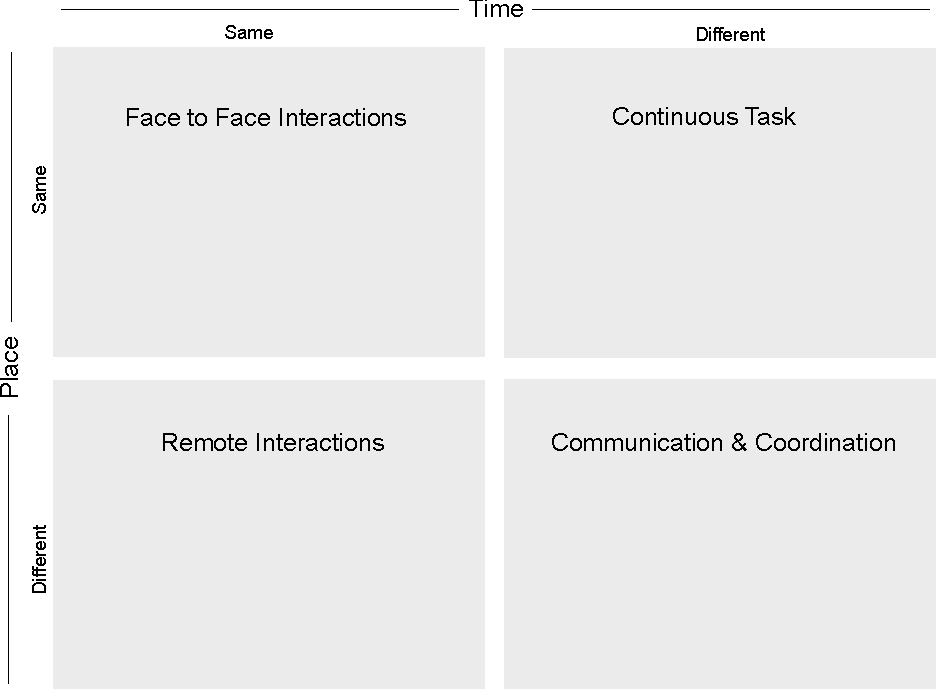
\includegraphics[width=0.8\columnwidth]{images/cscw_time_place_matrix.pdf}
 \caption[CSCW Place/Time Matrix]{\gls{CSCW} Place/Time Matrix \citep{xx}}
\label{fig:images_cscw_time_place_matrix}
\end{figure}

Additionally it is possible to group the CSCW systems based on the 3C model: \\

\begin{figure}[H]
 \centering
 %\includesvg[width=0.5\columnwidth, svgpath = images/]{cscw_time_place_matrix}
 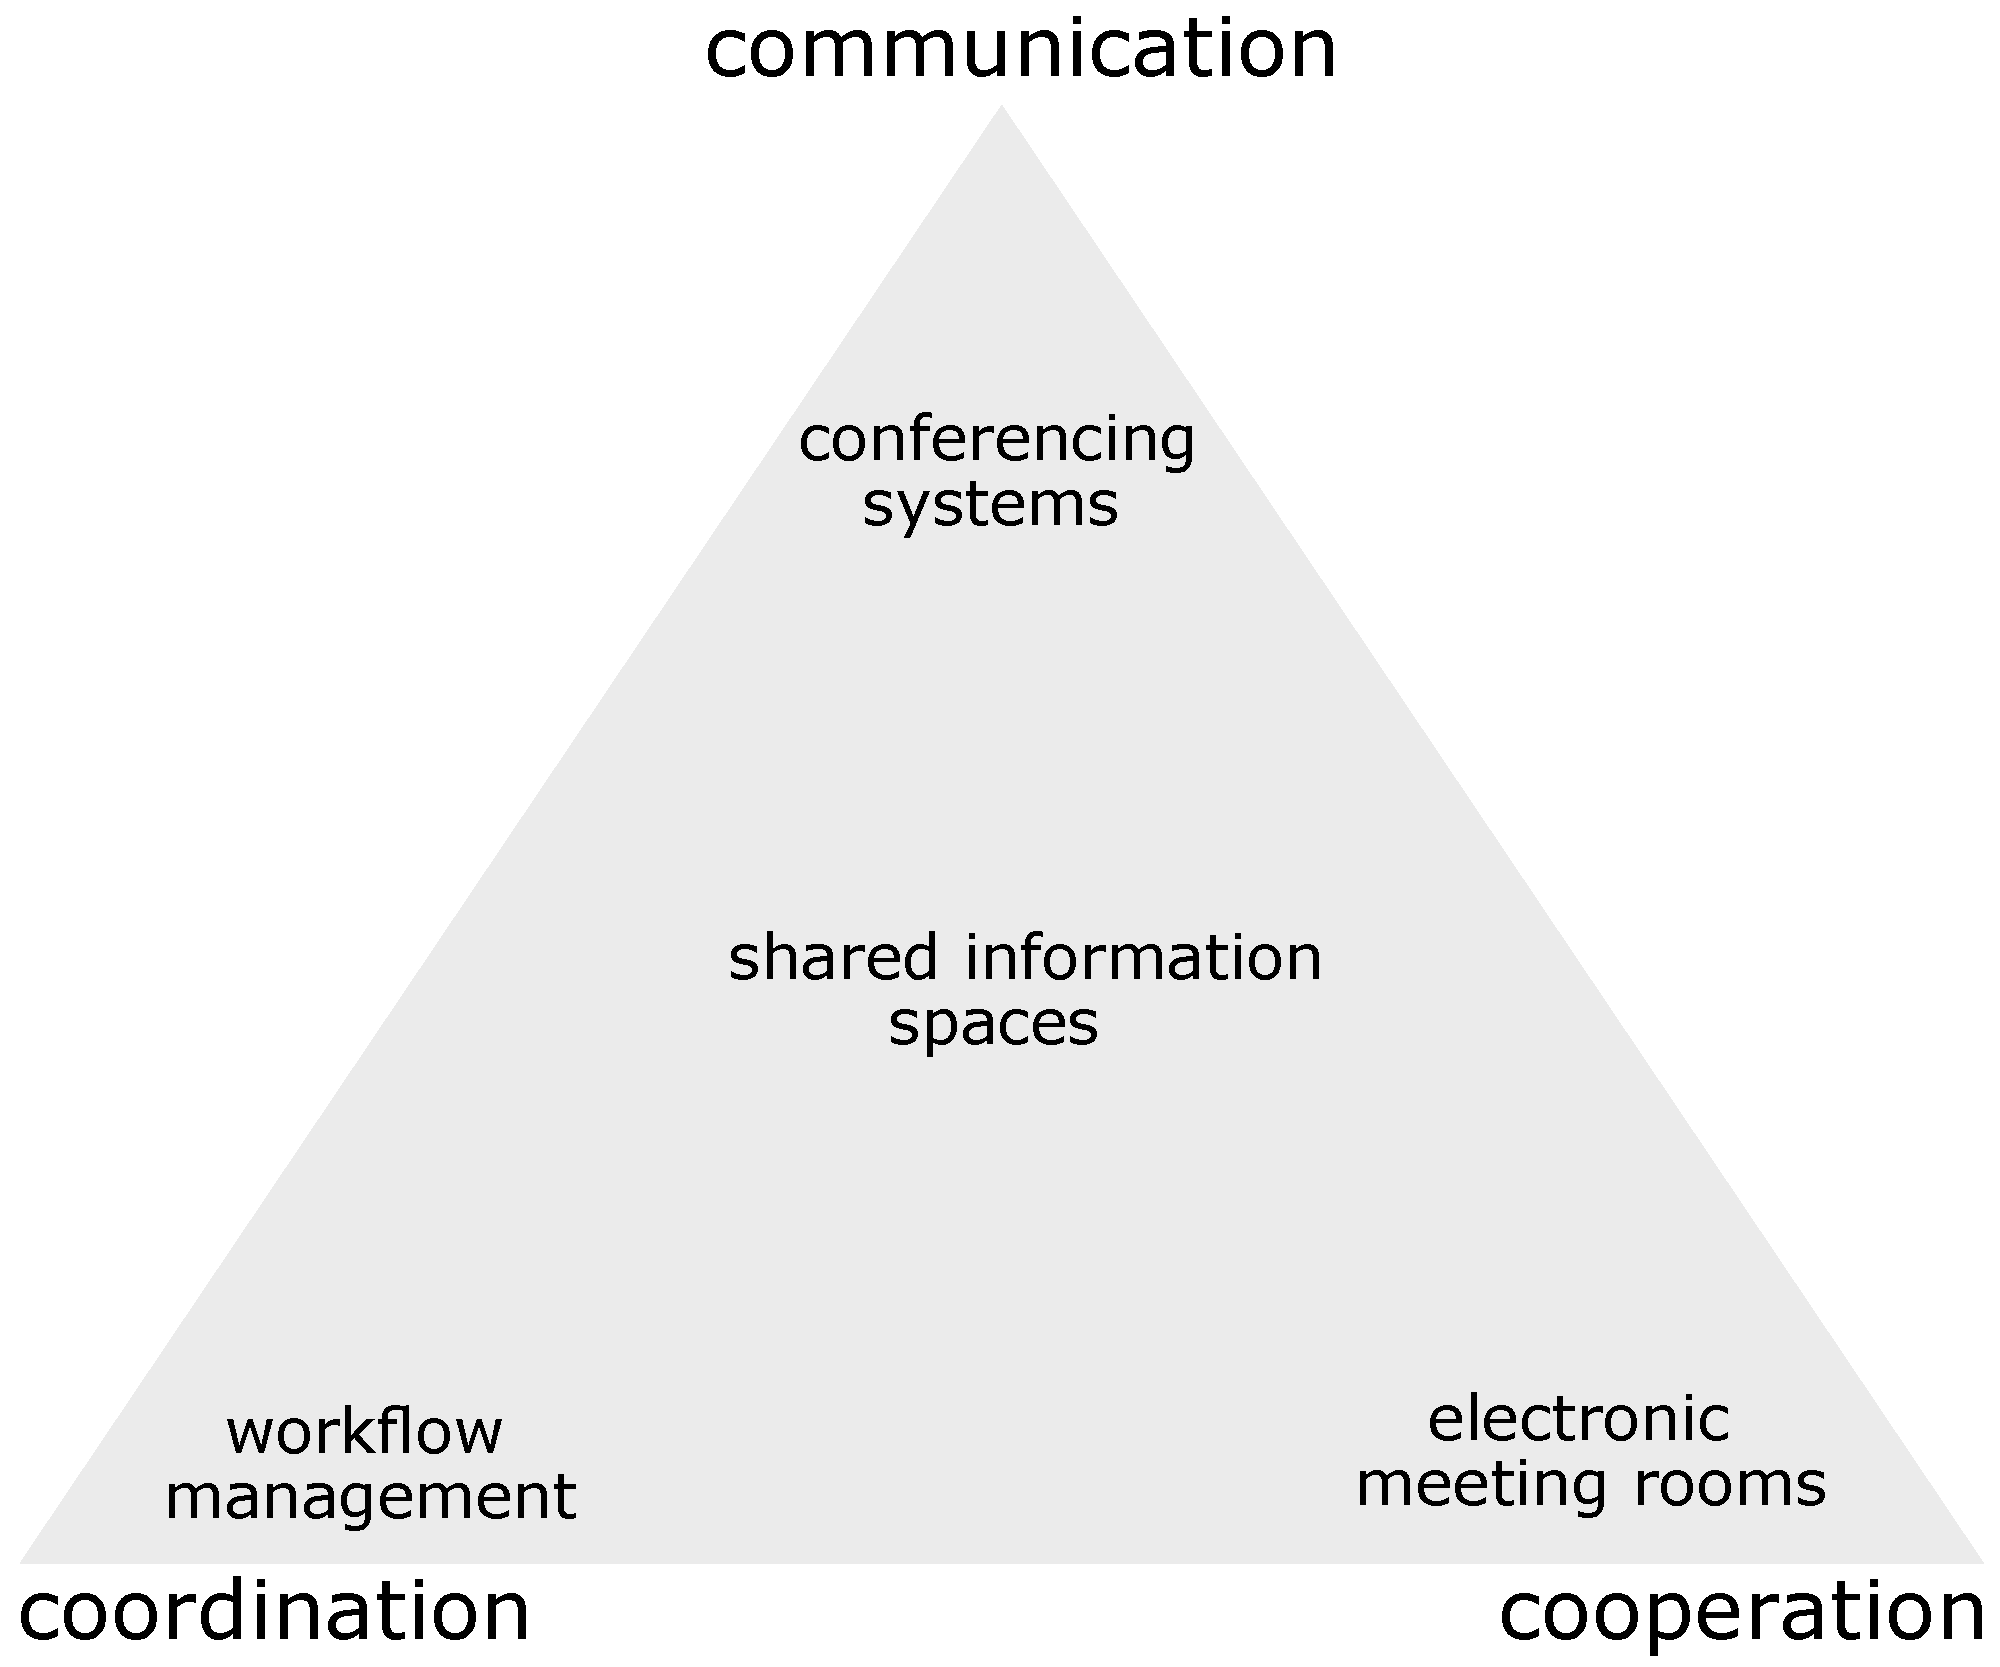
\includegraphics[width=0.8\columnwidth]{images/3C-model.pdf}
 \caption[The 3C Model]{The 3C Model \citep{Koch2008}}
\label{fig:images_cscw_3C_model}
\end{figure}

% section cscw_types (end)

\subsection{Shared Information Spaces}
\label{sec:cscw_shared_spaces}

% section cscw_shared_spaces (end)

\subsection{Important aspects of CSCW systems}
\label{sec:cscw_req_aspects}

% section cscw_req_aspects (end)

% section cscw (end)


% sub chapter semantic web
%!TEX root = ../MasterThesis.tex

\section{The Semantic Web}
\label{sec:semantic_web}

The \emph{Semantic Web} initiative strives for a better integration of distributed data from various publishers on the Web to enable new kinds of Smart Web applications. To achieve this goal, the Semantic Web delivers the infrastructure for this vision in form of various standard specifications such as \gls{RDF}, \gls{RDFS}, \gls{OWL}, \gls{SPARQL}, \ldots, which are introduced during the course of this section. Before going into the technical specifications of these the section shows the fundamental aspects underlying the (Semantic) Web as a whole.

\subsection{Fundamental aspects}
\label{subsec:fundamentals_semweb}

The Semantic Web builds on the fundamentals of the existing World-Wide Web, especially \citep[pg. 4-11]{allemang2011semantic}: \@

\begin{itemize}
	\item \textbf{AAA-Slogan:} Anyone can say Anything about Any topic. The Web does not restrict what people can post or publish on it. It is in the responsibilities of the readers to decide whether they can trust information from a specific source or not.
	\item \textbf{Open World Assumption:} as the amount of information on the Web is endless, and new information is published every day, one must always assume that there are new information available on it, that one does not know yet. As of this one can never be sure to have all facts at hand. New information can be published at any time that can give additional insights.
	\item \textbf{Non-unique Naming Assumption:} there is no central authority, who is responsible for providing unique identifiers for entities on the Web. Due to this fact different \gls{URI}s might refer to the same entity or real-world object.
\end{itemize}

Instead of making information on the Web available for human consumption \emph{only}, the Semantic Web is trying to make the information on the Web accessible (and readable) to machines as well. This will allow the integration of information across Web sites, and enable a distributed, interlinked ``Web of Data''. The major design principles to achieve this objective are \citep[pg. 1-22]{antoniou2008semantic}: \@

\begin{enumerate}
	\item make structured and semi-structured data available in standard formats,
	\item make individual data elements and their relationships accessible on the Web,
	\item describe the intended semantics of the data in a machine readable format
\end{enumerate}

The data model of the Semantic Web is build upon labeled graphs with objects and their relationships. Objects are modeled as nodes and their relationships as edges between them. To express these graphs of objects and their relationships, the Semantic Web: \@

\begin{itemize}
	\item formalize the syntax of the graph in \gls{RDF} (see Section~\ref{sec:semantic_rdf}),
	\item use \gls{URI}s to identify individual data items and relations (see Section~\ref{subsec:uri_concept}),
	\item use ontologies to represent semantics of the entities. Ontologies can be lightweight \gls{RDFS} definitions or expressive descriptions in the \gls{OWL} language (see Section~\ref{sec:semantic_ontologies}).
\end{itemize}

Initially it was tried to solve the data integration aspect on the Web with the exchange of \gls{XML} based messages, but though the \gls{XML} format is more machine-readable as \gls{HTML} it still lacks the semantic of the data transmitted (see Section~\ref{subsec:xml_format}). Therefore the Semantic Web defines the \gls{RDF} format as the basic data exchange format of it. Still the \gls{RDF} format was initially based on the \gls{XML} specification. To formally describe the existing terms and their relationships within a domain the Semantic Web relies on an ontology specification. These specifications are either expressed in \gls{RDFS} or uses the more expressive \gls{OWL} language; both of them are meta-description languages, which allows the definition of domain-specific knowledge representations based on the concepts found in \gls{RDF} itself. \\

As such the Semantic Web is a layered approach as depicted in Figure~\ref{fig:images_semweb_model}.\@

\begin{figure}[H]
	\centering
		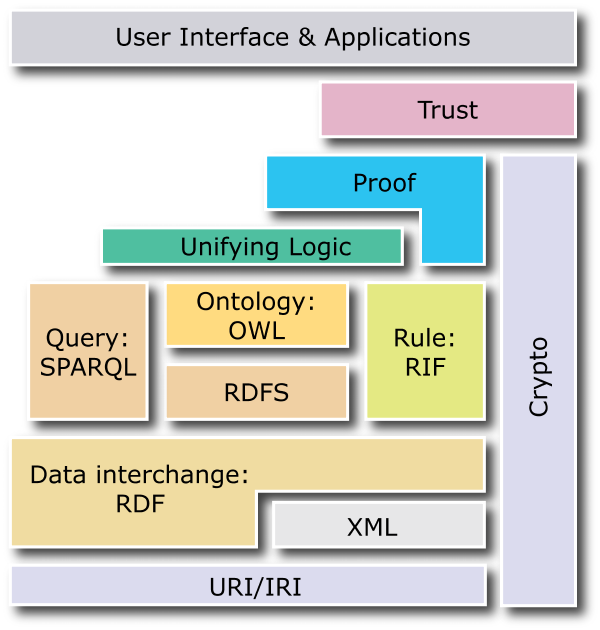
\includegraphics[width=0.8\columnwidth]{images/semantic_web_layers.png}
	\caption[The Semantic Web Model]{The Semantic Web Model \citep{W3C2013}}
\label{fig:images_semweb_model}
\end{figure}

% section semantic_fundamentals (end)

\subsection{Resource Description Framework}
\label{sec:semantic_rdf}

When trying to come up with a specification on how to integrate data on a globally dispersed platform such as the World-Wide Web, one will have to answer the following questions first: \@

\begin{itemize}
	\item \textbf{syntax:} How to serialize the data?
	\item \textbf{data model:} How to structure and organize the data?
	\item \textbf{semantics:} How to interpret the data?
\end{itemize}

Whereas the World-Wide Web is made up from interlinked documents in the \gls{HTML} format that is specifically designed for rendering information on screen to be consumed by a human, the \gls{RDF} brings a highly flexible data model to the Web. Its basic building block is the \emph{triple}, that is a statement consisting of an entity, an attribute and a value. The parts of a statement are also known as subject, predicate and object, which make up a directed graph as shown in the example in Figure~\ref{fig:images_semweb_triple}: \@

\begin{figure}[H]
	\centering
		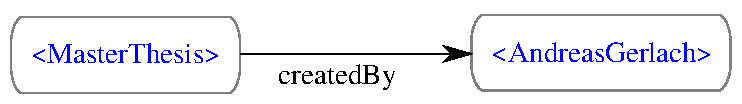
\includegraphics[width=0.8\columnwidth]{images/sample_triple.pdf}
	\caption{A basic example for a triple-statement}
\label{fig:images_semweb_triple}
\end{figure}

In this example the triple consists of the entity ``MasterThesis'', the assigned attribute ``createdBy'' and the value ``AndreasGerlach''. The value-part of a triple can contain either a literal value or another entity (as in the example above). Still a problem with this example statement is that the entities are not unique. Based on the given information it is not clear, which specific ``MasterThesis'' is meant and to whom the value ``AndreasGerlach'' refers. Additionally the predicate shown could have multiple meanings. These ambiguities have to be resolved on the Semantic Web to be able to make these information understandable by machines. To solve these issues the Semantic Web standard specifies that names of entities and predicates have to use a \gls{URI} (see Section~\ref{subsec:uri_concept}) to make their meanings clear. Literals that can be used as values such as numbers, dates and strings borrow their data type specifications from the \gls{XML} standard \citep[pg. 15-38]{wood2014linked}. \\

Based on this description the foundational elements of \gls{RDF} can be summarized as: \@

\begin{itemize}
	\item \textbf{entities:} aka resources or ``things'' of interest that are identified via \gls{URI}s
	\item \textbf{predicates:} aka attributes or properties that specify the relations between resources and are also identified by \gls{URI}s
	\item \textbf{literals:} integral values such as numbers, dates and strings that are based on the \gls{XML} data type specification
	\item \textbf{statements:} assign a value (either another entity or a literal) to a ``entity-predicate'' relation
	\item \textbf{graphs:} as the data model behind \gls{RDF} enables a  distributed, interlinked ``Web of Data''
\end{itemize}

\gls{RDF} triples can be serialized into four different syntax formats \citep[pg. 43-54]{wood2014linked}: \@

\begin{itemize}

	\item \textbf{\gls{RDF}/\gls{XML}:} the original format of the \gls{RDF} specification is based on the \gls{XML} specification. Because of their complexity they are best used with a parser program. For an example see Listing~\ref{lst:xml_meta_data}.
	\item \textbf{\gls{RDFa}:} describes how to embed \gls{RDF} information into existing \gls{HTML} documents. It allows Web site authors to enrich their Web pages with semantic information by adding a set of \gls{HTML} attributes to important items of the document. For an example see Listing~\ref{lst:rdfa_meta_data}.
	\item \textbf{\gls{JSON-LD}:} a recent initiative to allow JavaScript developers to use \gls{JSON} documents to express a \gls{RDF} statement, see Listing~\ref{lst:jsonld_meta_data}
	\item \textbf{Turtle:} a human readable serialization format for \gls{RDF} statements. \gls{URI}s can be shortened with a declared prefix, statements have to be finished with `.'. Statements referring to the same entity can be abbreviated via `;', which repeats the subject from the previous statement, or `,', which repeats subject and predicate from it. For an example see Listing~\ref{lst:turtle_meta_data}.
\end{itemize}

\begin{listing}[H]
	\begin{minted}[linenos,
	               numbersep=5pt,
	               breaklines=true,
	               frame=lines,
								 gobble=2]{XML}
		<?xml version="1.0"?>
		<rdf:RDF xmlns:rdfs="http://www.w3.org/2000/01/rdf-schema#"
			xmlns:ex="http://www.example.com/">
		  <rdf:Description rdf:about="http://www.example.com/MasterThesis">
		    <ex:createdBy rdf:resource="http://www.example.com/AndreasGerlach" />
		  </rdf:Description>
		</rdf:RDF>
	\end{minted}
\caption{A triple statement expressed in \gls{RDF}/\gls{XML} format}
\label{lst:xml_meta_data}
\end{listing}

\begin{listing}[H]
	\begin{minted}[linenos,
	               numbersep=5pt,
	               breaklines=true,
	               frame=lines,
								 gobble=2]{HTML}
	  <div about="http://www.example.com/MasterThesis">
	    <span rel="http://www.example.com/createdBy" resource="http://www.example.com/AndreasGerlach">
	  </div>
	\end{minted}
\caption{A triple statement expressed in \gls{RDFa} format}
\label{lst:rdfa_meta_data}
\end{listing}

\begin{listing}[H]
	\begin{minted}[linenos,
	               numbersep=5pt,
	               breaklines=true,
	               frame=lines,
								 gobble=2]{JSON}
  {
   "@context": "http://www.example.com/",
   "@id": "http://www.example.com/MasterThesis",
   "createdBy": "http://www.example.com/AndreasGerlach"
 	}
	\end{minted}
\caption{A triple statement expressed in \gls{JSON-LD} format}
\label{lst:jsonld_meta_data}
\end{listing}

\begin{listing}[H]
	\begin{minted}[linenos,
	               numbersep=5pt,
	               breaklines=true,
	               frame=lines,
								 gobble=2]{TURTLE}
	  @prefix ex:  <http://www.example.com/> .
	  ex:MasterThesis ex:createdBy ex:AndreasGerlach .
	\end{minted}
\caption{A triple statement expressed in Turle format}
\label{lst:turtle_meta_data}
\end{listing}

Coming back to the initial questions that have to be solved for data integration on a larger scale, this section showed how the Semantic Web tries to solve them, such as this: \@

\begin{itemize}
	\item \textbf{syntax:} supports the following formats: Turtle, \gls{RDFa}, \gls{RDF}/\gls{XML} and \gls{JSON-LD},
	\item \textbf{data model:} graph-based data model in \gls{RDF} specification,
	\item \textbf{semantics:} express semantics of the data in \gls{RDFS}. This will be the topic of the next section.
\end{itemize}

% section semantic_rdf (end)

\subsection{Web Ontologies}
\label{sec:semantic_ontologies}

Lightweight approach: RDFS \\
- is about adding semantics to your RDF documents \\
\\
Start by: \\
1. specify the \textbf{things} to talk about \\
   differentiate between \textit{objects} (real entities) and \textit{classes} (set of entities) \\
   `rdf:type' attribute to assign objects to classes (object = instance of this class) \\
   impose restrictions on the kind of properties used on objects: \\
   - restrictions on values are called `range' restrictions (object can take values of \ldots) \\
   - restrictions on property-object relations are called `domain' restrictions (this relation applies to objects of \ldots) \\
2. set up relations between classes (inheritance, composition) \\
3. define properties (registered globally) and the possible hierarchy relationship between them (global properties means you can
extend existing RDFS classes with your own properties easily) \\
\\
\begin{figure}[H]
	\centering
		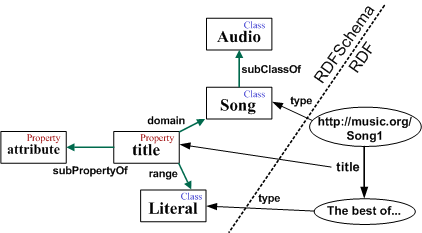
\includegraphics[height=2.5in]{images/RDFSchema.png}
	\caption{RDF Schema sample}
\label{fig:images_rdfs_sample}
\end{figure}

RDFS is described in RDF style using: \\
- core classes like: \\
  - `rdfs:Resource' (all objects/resources) \\
  - `rdfs:Class' (all classes) \\
  - `rdfs:Literal' (all literals) \\
  - `rdfs:Property' (all properties) \\
  - `rdfs:Statement' (all reified statements) \\
- core properties like: \\
  - `rdfs:type' (specify kind of class) \\
  - `rdfs:subClassOf' (specify inheritance between classes) \\
  - `rdfs:subPropertyOf' (specify inheritance between properties) \\
  - `rdfs:domain' (specify domain restrictions) \\
  - `rdfs:range' (specify range restrictions) \\
- container classes like: \\
  - `rdf:Bag'  (unordered list of entitites) \\
  - `rdf:Seq'  (ordered list of entities) \\
  - `rdf:Alt'  (list of alternatives/choices) \\
  - `rdf:Container' (superclass for all containers) \\
- utility classes like: \\
  - `rdfs:seeAlso', `rdfs:isDefinedBy' (links and references to other entities) \\
  - `rdfs:Comment' (comments and notes of entities) \\
  - `rdfs:Label' (human-friendly name of entities) \\
\\

Missing features in RDFS: \ldots  \\
\\
Complex Ontologies in Web Ontology Language (OWL): \\
\ldots \\
\\

% section semantic_ontologies (end)

\subsection{Query Language}
\label{sec:semantic_querylang}

SPARQL requires a \textbf{triple store} - a database containing RDF documents \\
is also referred to as a \textit{Graph Store} \\
data is inserted via Bulk load operation or via SPARQL update statements \\
SPARQL consist of SPARQL Queries that are send over the SPARQL protocol \\
Clients sends the queries to an HTTP endpoint \\
Stores on the public Web incl. dbpedia.org, ckan.org, wikidata.org \\
SPARQL also works with RDFS \\
SPARQL has similarities to SQL:
- each element in a triple might be replaced with a variable like `?varName' like so: \\

\begin{listing}[H]
	\begin{minted}[linenos,
	               numbersep=5pt,
	               gobble=2,
	               frame=lines,
	               framesep=2mm]{SPARQL}
	  PREFIX ns1:<URI>
	  PREFIX ns2:<URI>
	  PREFIX ns3:<URI>

	  SELECT ?varName
	  WHERE {
	      ns1:subject ns2:predicate ?varName
	  }
	\end{minted}
\caption{Selecting information with \gls{SPARQL}}
\label{lst:select_sparql}
\end{listing}

- in the WHERE clause it hosts the graph pattern to match (could be cascaded to go down subgraphs) \\
- variables can occur at any place in the graph pattern (?subj ?pred ?obj) as select with query everything \\
\\
LIMIT \textless n\textgreater option at the end for limiting the result set \\
FILTER (?varName \textless condition\textgreater ) in graph pattern can restrict results to match some
literal values and supports: \\
- numbers, dates: \textless, \textgreater, = \\
- strings: =, regex() \\
\\
\textbf{open world} assumption: resources on the Web are described in different schematas with various properties
using different vocabularies \\
- UNION option in graph pattern combines different matches \\
- OPTIONAL option in graph pattern only returns those entities if they are available (otherwise empty) \\
\\
ASK query checks for the existence of a given graph pattern \\
CONSTRUCT can be used to retrieve a subgraph from a larger graph, can also be used to translate between different schemas \\

\begin{listing}[H]
	\begin{minted}[linenos,
	               numbersep=5pt,
	               gobble=2,
	               frame=lines,
	               framesep=2mm]{SPARQL}
	  PREFIX ns1:<URI>
	  PREFIX ns2:<URI>
	  PREFIX ns3:<URI>

	  CONSTRUCT {
	      ?varA ns2:predicate ?varB .
	      ?varA ns3:predicate ?literalA .
	  }
	  WHERE {
	      ?varA ns1:predicate ?varB
	  }
	  FILTER ( ?varB > x )
	\end{minted}
\caption{A CONSTRUCT query in \gls{SPARQL}}
\label{lst:construct_sparql}
\end{listing}

- SPARQL can be used to harmonize graphs from different sources \\
- is also used for basic reasoning ala ``if found this, assume that'' \\
- can ease hierarchical queries with * or + on the predicate (SPARQL 1.1) \\
- can help resolving issues with different entities referring to the same object (MKP pg. 95)\\
- Federated Queries can be used to combine information from distinct sources via SPARQL (MKP pg. 110-112)\\
\\
- inferencing information from existing triples via SPIN (SPARQL Inferencing Notation) \\
- like in a taxonomy items can be categorized in an hierarchy (MKP pg. 114) \\
- inference patterns are used in Semantic Web applications (MKP pg. 115) \\
   * subClassOf - type propagation rule \\
- inferencing could be done at query time or persistently (MKP pg. 120/121) \\
- inferences can also be helpful when combining information from unknown sources \\
- inferencing happens on various levels (RDFS, RDFS+, OWL) with an increased set of complex inferencing rules (MKP pg. 122/123)
\\
% section semantic_querylang (end)

\subsection{Agents and Rules}
\label{sec:semantic_logic_rules}


% section semantic_logic_rules (end)

% section semantic_web (end)


% sub chapter peer-to-peer communications
%!TEX root = ../MasterThesis.tex

\section{Peer-to-peer communication}
\label{sec:p2p_communication}

This section explains the core concepts of \gls{P2P} communication technologies. It begins with a comparison of the benefits and disadvantages of centralized and decentralized Web architectures. After that it shows how \gls{P2P} communication networks can be structured, the different ways to initiate a communication session as well as how data can be transmitted between peers.

\subsection{Centralized vs. Decentralized Web architectures}
\label{sec:central_decentral_arch}

In classical client-server applications the information is stored on a central system (aka server). Clients have to connect to the server and ask for the information. The server handles the requests from the clients and deliver the information in case a request was valid. Prominent examples of centralized Web architectures are Social Networks such as Facebook or Twitter, in which clients, such as a Web browser or Mobile application, communicate with a Web service that runs on a server of the organization providing these Social Networks, to access and retrieve Web documents (e.g.\ \gls{HTML}, images, audio, video, \ldots) via the \gls{HTTP} protocol, as shown in Figure~\ref{fig:p2p_central_server}. \@

\begin{figure}[H]
	\centering
		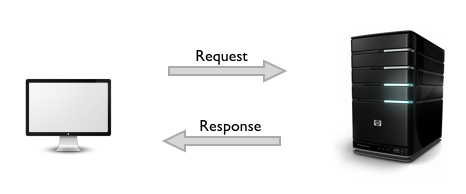
\includegraphics[width=0.9\columnwidth]{images/client-server-web.png}
	\caption[Centralized Web architectures as used by prominent Social Networks]{Centralized Web architectures as used by prominent Social Networks \citep{codeTuts}}
\label{fig:p2p_central_server}
\end{figure}

As a consequence of this architecture all of the information are centralized and under control of the provider of the (Web) service. This can lead to a variety of problems, including serious issues such as unreliable or no longer existing services will result in a dismissal of all the information stored on them, or privacy concerns for user-generated content stored on those central servers. \\

In opposite to that a \gls{P2P} network considers all nodes as equal. This offers the benefits that information can be kept on each node, and each node can provide access to its information to any other node on the network. Due to this the \gls{P2P} system has an high degree of decentralization, is not owned and controlled by a specific company, and therefore tends to me more resilient to faults, outages and attacks. But due to the distributed nature of it, looking for and accessing information is more difficult. Information in a \gls{P2P} system have to be indexed in a way so that the correct node is queried for it. Still this index has to be stored somewhere in the system, and the optimal solution for the indexing problem depends on the type of \gls{P2P} system used (see next section). Additionally, the way new nodes get connected to the system is depending on the type of \gls{P2P} system used, and might lead to the introduction of special bootstrap or super nodes into the network as shown in Figure~\ref{fig:p2p_overlay_network} \citep{parameswaran2001p2p}.

\begin{figure}[H]
	\centering
		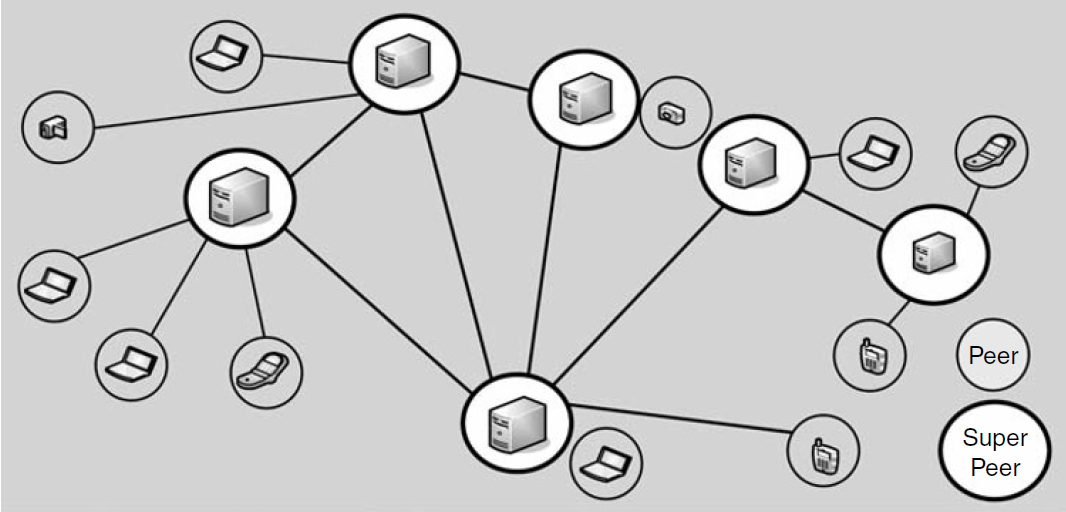
\includegraphics[width=0.8\columnwidth]{images/p2p_network.png}
	\caption[A \gls{P2P} overlay network]{A \gls{P2P} overlay network \citep[pg. 9]{buford2009p2p}}
\label{fig:p2p_overlay_network}
\end{figure}

% section central_decentral_arch (end)

\subsection{Classification of \gls{P2P} systems}
\label{sec:p2p_classification}

\gls{P2P} system architectures can be classified based on their degree of centralization into: \@

\begin{itemize}
	\item \textbf{partially centralized \gls{P2P} system:} rely on a dedicated controller node that maintains the set of participating nodes, host the index of the information available in the system, and controls the overall operation of the network,
	\item \textbf{decentralized \gls{P2P} system:} does not use any dedicated controller node, but may need to introduce bootstrap and super nodes for maintaining the list of participating nodes and the index of the information available depending on the size of the network.
\end{itemize}

\begin{figure}[H]
	\centering
		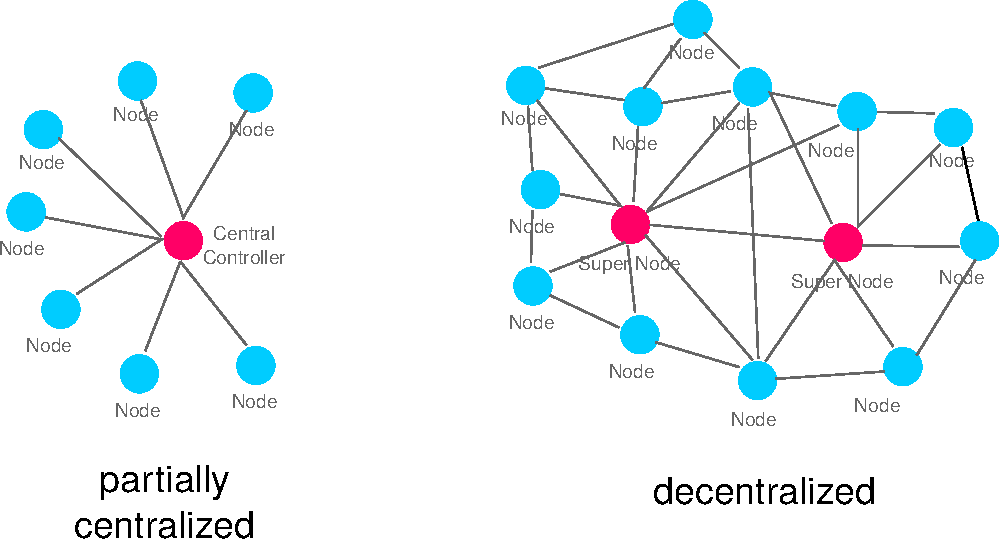
\includegraphics[width=0.8\columnwidth]{images/p2p_network_structures.pdf}
	\caption{Classification of \gls{P2P} networks}
\label{fig:p2p_network_structures}
\end{figure}

% section p2p_classification (end)

\subsection{Communication in a \gls{P2P} network}
\label{sec:p2p_start_communication}

The procedure to establish a \gls{P2P} communication depends on the structure of the \gls{P2P} system. In a \emph{partly centralized \gls{P2P} system} new nodes join the network by connecting to the central controller first. This central controller has a well-known \gls{IP} address and maintains the operation of the whole \gls{P2P} network. Due to this, any new node has to register with the central controller to get introduced to the \gls{P2P} network. The controller also maintains the information about the overlay network as well as the information about each object and on which node(s) it resides within the network. The overlay is typically following a star-shaped topology with the central controller at the center, see Figure~\ref{fig:p2p_network_structures}. \\

In a \emph{decentralized \gls{P2P} system} new nodes are expected to obtain the \gls{IP} address they have to connect to initially via a separate channel (e.g.\ as a link on a Web site). Depending on the size of the \gls{P2P} network additional bootstrap or super nodes, which help to set up a new node, are available on the network. These special nodes are generally also consolidating information about the objects available on the peers nearby, which helps speeding up searching and accessing required information. The overlay information of such a distributed network can be either \emph{structured}, in which each node receives a unique identifier from a numeric keyspace resembling the responsibilities of that node, or \emph{unstructured}, in which there is no particular network structure, and no further constraints are assigned to the nodes of the network. \\

A \emph{structured overlay} maintain the information within the network more efficiently, because it uses a distributed hash-table to maintain a distributed index and decides the location (aka node) of an object in the network based on its hash-value. In an \emph{unstructured overlay network} the information is typically stored on the node that introduces it. To locate an object a query request is typically broadcasted through the overlay network. Based on the size of the network and the distance between the node asking for and the node holding the information querying and accessing an information on an unstructured overlay network can take some time, and can also flood the whole network with query requests. Therefore, requesting nodes often set the scope of the request, which limits the number of hops that should be done on the network. This will reduce the communication overhead on the whole system. Additionally, introducing super nodes that collect and maintain indexes of their peers nearby can further reduce the number of hops necessary to find the required information, see Figure~\ref{fig:p2p_network_structures} \citep{rodrigues2010peer}. \@

% section p2p_start_communication

\subsection{The \gls{WebRTC} standard}
\label{sec:p2p_webrtc}

``Web Real-Time Communication (\gls{WebRTC}) is a collection of standards, protocols, and JavaScript \gls{API}s, the combination of which enables peer-to-peer audio, video, and data sharing between browsers (peers)'' \citep[pg. 307]{grigorik2013high}. Although this new \gls{W3C} standard usually stands for in-browser video or audio conferencing without the need of proprietary browser extensions, it also offers ways to exchange arbitrary messages or binary data between participating peers in a distributed Web application. Due to being an open Web standard \gls{WebRTC} is available in many current Web browsers directly, and is widely adopted as a standardized and open way to establish a \gls{P2P} communication between clients of a Web site, or from within a Web application. The standard wraps a lot of the complexities of establishing peer-to-peer communication channels and transmitting data into three primary \gls{API}s \citep[pg. 307-308]{grigorik2013high}: \@

\begin{itemize}
	\item \textbf{MediaStream:} for acquiring access to and retrieve data from local audio and video devices,
	\item \textbf{RTCPeerConnection:} for establishing a peer-to-peer connection between clients,
	\item \textbf{RTCDataChannel:} for transmitting arbitrary application data
\end{itemize}

To establish a data connection between peers a Web application has to create a RTCPeerConnection object first, before it can create a RTCDataChannel to exchange messages on it. Establishing a \gls{P2P} connection between globally dispersed peers on the Web is not a trivial task and has to provide fallback solutions in case of \gls{P2P} connectivity issues due to firewall or \gls{NAT} services used by some of the peers, which usually prevent clients to connect to each other directly. Fortunately, the \gls{W3C} standard is taking care of these steps during the initiating of a \gls{WebRTC} connection by utilizing the \gls{ICE} protocol. After being able to open a connection to another peer, a communication session has to be created. For that the communicating peers have to negotiate on protocols, encodings, and additional functionality required for the \gls{P2P} communication tasks at hand. The \gls{WebRTC} uses the \gls{SCTP} to exchange application data between peers \citep[pg. 315-330]{grigorik2013high}. It has the following set of features \citep[pg. 342]{grigorik2013high}: \@

\begin{itemize}
		\item \textbf{Reliability:} the data channel can be configured to use either reliable or unreliable delivery of packages,
		\item \textbf{Delivery:} the data channel can be also configured to support either in-order or out-of-order delivery of packages,
		\item \textbf{Transmission:} the transport of data is message-oriented,
		\item \textbf{Confidentiality/Integrity:} all application data transmitted between the peers is encrypted to guarantee confidentiality and integrity of the data exchanged.
\end{itemize}

For a purely data transmission channel one can also disable any audio and video transfers during the setup of the communication session (see Listing~\ref{lst:p2p_webrtc_data_only}). \@

\begin{listing}[H]
	\inputminted[linenos,
							 numbersep=5pt,
							 breaklines=true,
							 frame=lines]{JavaScript}
		{./samples/initiateWebRTCConnection.js}
\caption[Establishing a pure \gls{WebRTC} data connection]{Establishing a pure \gls{WebRTC} data connection \citep[pg. 349]{grigorik2013high}}
\label{lst:p2p_webrtc_data_only}
\end{listing}

Once a data channel has been established between the peers application data can be exchanged between them via message passing, as shown in Listing~\ref{lst:p2p_webrct_data_send}: \@

\begin{listing}[H]
	\inputminted[linenos,
							 numbersep=5pt,
							 breaklines=true,
							 frame=lines]{JavaScript}
		{./samples/handleWebRTCDataChannel.js}
\caption[Message-oriented communication via a \gls{WebRTC} data channel]{Message-oriented communication via a \gls{WebRTC} data channel \citep[pg. 346]{grigorik2013high}}
\label{lst:p2p_webrct_data_send}
\end{listing}

% section p2p_webrtc (end)

% section p2p_communication (end)


% chapter theoretical foundations (end)


% The counter for tables and figures are set back in order to start a new numeration per chapter
\setcounter{table}{1}
\setcounter{figure}{1}
  % Inclusion of the forth chapter
  %!TEX root = ../MasterThesis.tex

\chapter{Design of a collaborative system} % (fold)
\label{cha:system_design}

This chapter about the design of a collaborative system to support the investigation of \gls{E-commerce} fraud incidents will start with a discussion of the semantics of the underlying \gls{RDF} data sets, and how these can be combined across various organizations. After that it shows how these information can be provided to the relevant parties based on the \gls{E-commerce} fraud investigation scenario described in Chapter~\ref{cha:context_analysis}. For this purpose it will have a detailed look into the partially centralized \gls{P2P} communication architecture and show how that can be used within the system for securely sharing the relevant information.

% sub chapter selecting a data schema
%!TEX root = ../MasterThesis.tex

\section{\gls{RDF} vocabularies and Web Ontologies for \gls{E-commerce}}
\label{sec:choose_data_schema}

As a major objective of the \gls{E-commerce} fraud investigation system is to collect the various transactional information from online merchants, \gls{PSP}s and issuers, combine and link them together, as well as analyse the resulting data set from different view points to find abnormal activities, the information exchanged between the relevant participants either have to follow commonly available \gls{RDF} vocabularies, have to be based on a custom shared \gls{RDF} vocabulary that has been specifically designed for this system, or have to be mapped and linked against each other from different \gls{RDF} schema specifications.

\subsection{Reuse of common \gls{RDF} vocabularies}
\label{subsec:reuse_vocab_web}

One valid approach to come up with a data schema for the collaborative system is to take a look into commonly used \gls{RDF} vocabularies and Web ontologies, and try to figure out whether they can be used for describing the information that need to be exchanged between participants of the \gls{E-commerce} fraud investigation system. When consulting the Semantic Web community for commonly agreed upon and highly used \gls{RDF} schema specifications, one will come up with the following list (see Table~\ref{tab:used_vocab_rdf}):\@

\begin{table}[H]
\centering
\begin{tabular}{p{3cm}llp{4.5cm}}
\hline
\textbf{Name} & \textbf{Prefix} & \textbf{Describes} & \textbf{Namespace URI} \\
\hline
Dublin Core & dc: & Meta data & \url{http://purl.org/dc/terms/} \\
\hline
FOAF & foaf: & People & \url{http://xmlns.com/foaf/0.1/} \\
\hline
Geo & pos: & Positions & \url{http://www.w3.org/2003/01/geo/wgs84\_pos\#} \\
\hline
Geo Names & gn: & Locations & \url{http://www.geonames.org/ontology\#} \\
\hline
Good Relations & gr: & Products & \url{http://purl.org/goodrelations/v1\#} \\
\hline
RDF & rdf: & Core framework & \url{http://www.w3.org/1999/02/22-rdf-syntax-ns\#} \\
\hline
RDFS & rdfs: & RDF vocabularies & \url{http://www.w3.org/2000/01/rdf-schema\#} \\
\hline
Schema.org & schema: & Schema.org vocabularies & \url{http://schema.org/} \\
\hline
SKOS & skos: & Controlled vocabularies & \url{http://www.w3.org/2004/02/skos/core\#} \\
\hline
vCard & vcard: & Business Cards & \url{http://www.w3.org/2006/vcard/ns\#} \\
\hline
Web Ontology Language & owl: & Ontologies & \url{http://www.w3.org/2002/07/owl\#} \\
\hline
XML Schema Datatypes & xsd: & Data types & \url{http://www.w3.org/2001/XMLSchema\#} \\
\hline
\end{tabular}
\caption[Commonly used \gls{RDF} vocabularies on the Web]{Commonly used \gls{RDF} vocabularies on the Web \citep[pg. 41]{wood2014linked}}
\label{tab:used_vocab_rdf}
\end{table}

Based on these existing schema specifications describing a fictive consumer named ``Max Mustermann'' \gls{incl}\ his home address can be done by combining data utilizing the \gls{FOAF} and \gls{vCard} vocabularies into a \gls{RDF} data set such as described in Listing~\ref{lst:sample_customer_mustermann} and visualized as directed graph in Figure~\ref{fig:images_sample_customer}. The described resource is uniquely identified by the \gls{URI} \url{http://www.merchant1.com/customers/MaxMustermann}. Additionally, one can see that these vocabularies use expressive names for their entities and predicates, which make it easier to understand their intended meanings (e.g.\ ``foaf:givenname'', ``vcard:locality'', \ldots).  \@

\begin{listing}[H]
  \inputminted[linenos,
               numbersep=5pt,
               breaklines=true,
               frame=lines]{TURTLE}
               {./samples/sample_customer_mustermann.ttl}
  \caption{Personal related information about a fictive consumer in \gls{RDF}}
\label{lst:sample_customer_mustermann}
\end{listing}

\begin{figure}[H]
	\centering
		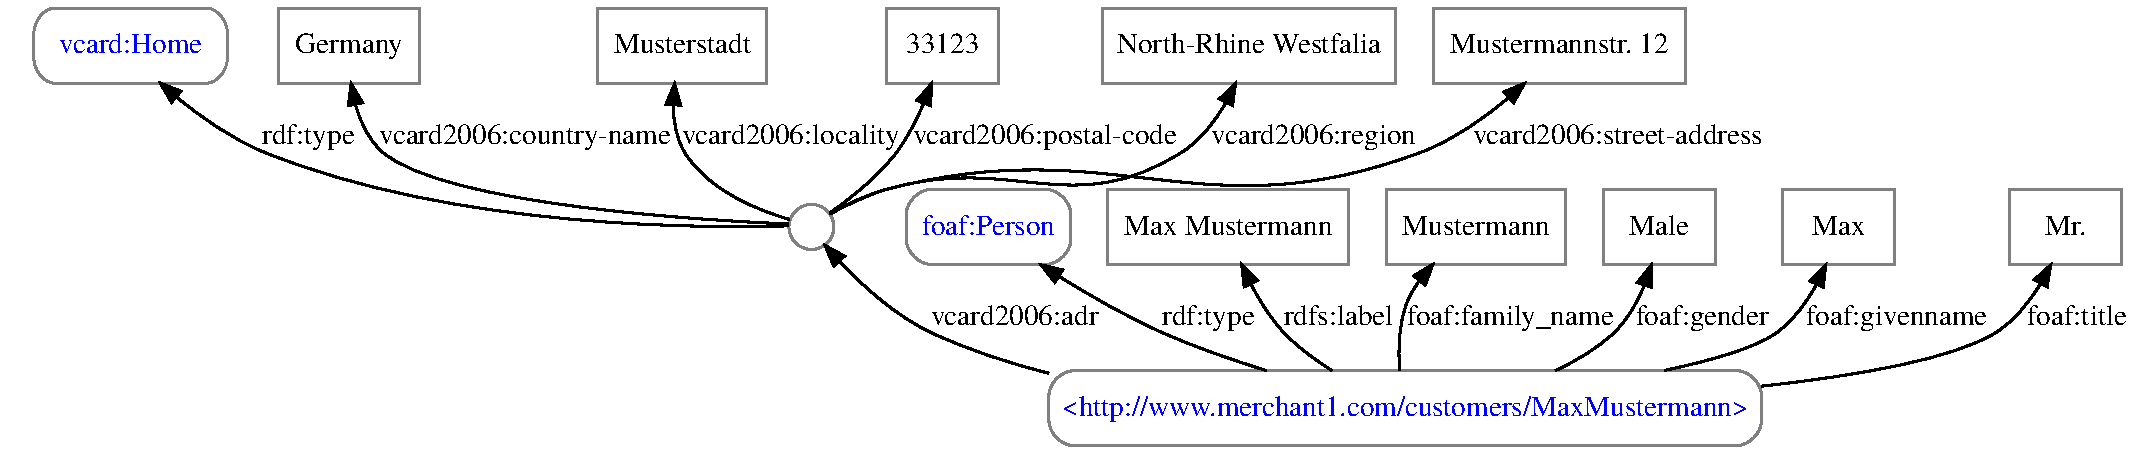
\includegraphics[width=\columnwidth]{images/sample_customer_mustermann.pdf}
	\caption{Graph representation of consumer information from Listing~\ref{lst:sample_customer_mustermann}}
\label{fig:images_sample_customer}
\end{figure}

However, being able to describe persons and their addresses is just a subset of the entities and relations found in the \gls{E-commerce} scenario. When looking back to the initial \gls{ER} model of an \gls{E-commerce} transaction as shown in Section~\ref{sec:data_model_transactions}, one can map the entities that are currently available in the \gls{E-commerce} scenario to the existing \gls{RDF} vocabularies such as follows (see Table~\ref{tab:map_tx_rdf_vocab}): \@

\begin{table}[H]
\centering
\begin{tabular}{p{5cm}l}
\hline
\textbf{Information} & \textbf{RDF vocabulary} \\
\hline
Consumer & FOAF \\
\hline
Credit Card Owner & FOAF \\
\hline
Billing Address & vCard \\
\hline
Shipping Address & vCard \\
\hline
Location Information & Geo Names \\
\hline
Merchant & GoodRelations \\
\hline
Items & GoodRelations \\
\hline
Item Categories & GoodRelations \\
\hline
Brands & GoodRelations \\
\hline
Payment Types & GoodRelations \\
\hline
\end{tabular}
\caption{Possible usage of \gls{RDF} vocabularies for \gls{E-commerce} transaction information}
\label{tab:map_tx_rdf_vocab}
\end{table}

As this table shows, there are some parts of the \gls{E-commerce} \gls{ER} model that can be expressed with existing \gls{RDF} vocabularies extensively such as personal related information via \gls{FOAF} and \gls{vCard}, whereas other parts can not be stated in-depth (e.g.\ credit card information), or are not specified at all (e.g.\ tracking of the delivery). Due to these circumstances, one usually have to build an own \gls{RDF} vocabulary or Web ontology that fills in the missing pieces, and refers to the existing concepts whenever appropriate.\\

When trying to model the information of a credit card as displayed in Figure~\ref{fig:images_data_model}, a possible result will be the \gls{RDFS} specification shown in Listing~\ref{lst:credit_card_vocab}. This definition of a credit card resource explicitly reuses entities from the \gls{FOAF} and GoodRelations ontologies by defining that: \@

\begin{itemize}
 \item the owner of a credit card has to be of type ``Person'' from the \gls{FOAF} ontology,
 \item the type of a credit card has to be an instance of the type ``PaymentMethodCreditCard'' from the GoodRelations ontology.
\end{itemize}

As most of the parts of the \gls{E-commerce} data model shown in Figure~\ref{fig:images_data_model} can not be expressed with the existing \gls{RDF} vocabularies directly, filling in the gaps would mean to come up with a large set of custom entities and relationships, which will limit the usage of the system as explained in Section~\ref{subsec:build_ontology_frauds}.

\begin{listing}[H]
 \inputminted[linenos,
              numbersep=5pt,
              breaklines=true,
              frame=lines]{TURTLE}
              {./samples/vocab_credit_card.ttl}
 \caption{A specification for a credit card in \gls{RDFS}}
\label{lst:credit_card_vocab}
\end{listing}

When analysing the list of existing and actively used \gls{RDF} vocabularies and Web ontologies in Table~\ref{tab:used_vocab_rdf}, one will also find the Schema.org initiative \citep{Schema.org}. This meta data vocabulary was initially designed by the leading search engines (e.g.\ Google, Microsoft and Yahoo!) to allow authors of Web sites to markup their \gls{HTML} documents in a way, so that they are better understood by these search engines. The Schema.org vocabulary is actively maintained by its community, includes new concepts with each release, and also offers an extension mechanism to implement additional vocabularies with terms that are not part of the core specifications \citep{SchemaExtensions} yet. In one of the past releases the maintainers also introduced all of the existing concepts of the GoodRelations ontology into the Schema.org vocabulary \citep{SchemaGoodRelation}. \\

As online merchants likely provide semantic meta data for their products and offerings in the vocabulary of Schema.org with the objective to improve their listings on search engine results (also known as \gls{SEO}) already, one can reuse parts of these information for the \gls{E-commerce} fraud investigation scenario. Additionally, the wide-ranging scope of aspects declared in the Schema.org vocabulary can make it a good fit for the collaborative system to support the investigation of \gls{E-commerce} frauds. When trying to map the initial \gls{ER} model from Section~\ref{sec:data_model_transactions} to the Schema.org core specifications, one will basically come up with a schema as displayed in Figure~\ref{fig:images_schema_org}. \@

\begin{figure}[H]
	\centering
		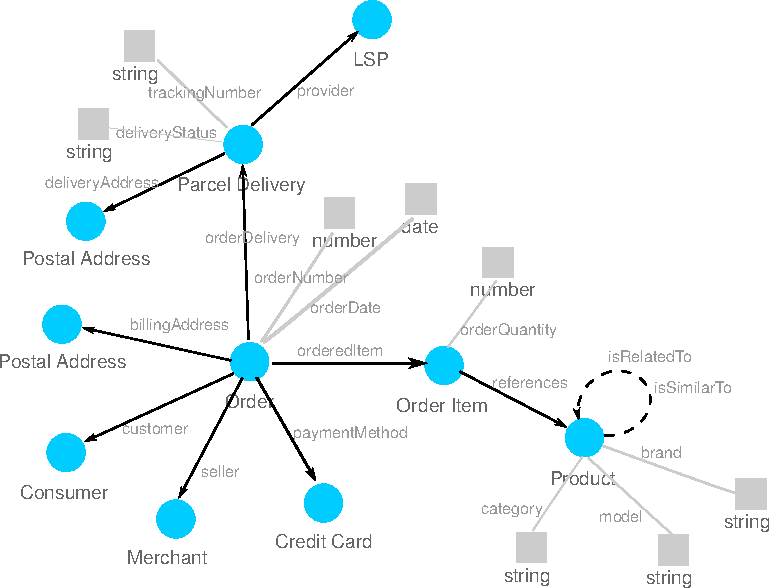
\includegraphics[width=0.8\columnwidth]{images/schema_org_mapping.pdf}
	\caption{Schema.org based mapping of an \gls{E-commerce} transaction}
\label{fig:images_schema_org}
\end{figure}

% subsection reuse_vocab_web (end)

\subsection{Creation of a custom \gls{RDF} vocabulary}
\label{subsec:build_ontology_frauds}

Another possible approach to harmonise information in the collaborative system is to define a completely new \gls{RDF} vocabulary or Web ontology for the proposed \gls{E-commerce} fraud investigation system, and share that with every possible stakeholder. This specification will have to define all the entities and relations known to the collaborative system and describe them in \gls{RDFS} format (see Section~\ref{sec:semantic_web}). \\

A major drawback of this approach is that new participants of the system will have to implement the conversion of their internal data structures to a \gls{RDF} data set that follows the predefined schema definition first, before even being able to join in. This will limit the general usage of the collaborative system, and will therefore not further considered in detail.

% subsection build ontology (end)

\subsection{Mapping of \gls{RDF} vocabularies}

Although it is possible to model an \gls{E-commerce} transaction solely with the Schema.org specifications as shown in Figure~\ref{fig:images_schema_org}, the collaborative system likely has to take care of the mapping of the transactional information coming from various sources to be able to combine them later. As the Semantic Web does not restrict how organizations structure and express their information, and due to the ``AAA slogan'' (see Section~\ref{sec:semantic_web}), there are likely different \gls{RDF} representations of an \gls{E-commerce} transaction in-use and have to be brought together. \\

The \gls{W3C} standards for the Semantic Web also include support for these mapping issues, because they will also come up when trying to combine semantic information available around the Web. The following axioms are available in the \gls{RDFS} and \gls{OWL} specifications explicitly for that purpose: \@

\begin{itemize}
	\item \textbf{rdfs:subClassOf:} a relation of type ``rdfs:subClassOf'' defines a specialization of a class, in which the child class inherits all the properties of the parent class,
  \item \textbf{rdfs:subProperyOf:} a relation of type ``rdfs:subPropertyOf'' defines a specialization of a property, in which the child property inherits all constraints of the parent property,
  \item \textbf{owl:equivalentClass:} a relation of type ``owl:equivalentClass'' specifies the equality of classes coming from different \gls{RDF} vocabularies or Web ontologies,
  \item \textbf{owl:equivalentProperty:} a relation of type ``owl:equivalentProperty'' specifies the equality of classes coming from different \gls{RDF} vocabularies or Web ontologies
\end{itemize}

If a merchant wants to state that a product related information, which is delivered as resource using the GoodRelations vocabulary, is equal to product information that can be found in the Schema.org specification, he or she can do so as follows (see Listing~\ref{lst:schema_mapping_gr_schema_org}): \@

\begin{listing}[H]
 \inputminted[linenos,
              numbersep=5pt,
              breaklines=true,
              frame=lines]{TURTLE}
              {./samples/mapping_gr_schema_org.ttl}
 \caption{Mapping product-related information from GoodRelations to Schema.org}
\label{lst:schema_mapping_gr_schema_org}
\end{listing}

These mapping statements from one \gls{RDF} vocabulary to another can be either created and injected into a \gls{RDF} data store by the party, who is going to merge information from different sources according to needs, or can also be part of the resource specification coming from an external source. In the former case the stakeholder, who is collecting and combining the information from various sources, has to maintain the additional triples to map information between each \gls{RDF} vocabulary used, and include them in the processing of the external statements within the combined \gls{RDF} data store. With an increased number of participants, which are using disjunct \gls{RDF} vocabularies, the effort and time to manage and create these mapping instructions on the collectors side will increase tremendously. Thus, the second approach is the preferred one. In that situation the \gls{RDF} description of an entity coming from an external source is already stating the mapping to one or more well-known \gls{RDF} vocabularies (e.g.\ the Schema.org specification mentioned above). This will reduce the effort and time to combine the information from different sources, and will only slightly increase the effort on the side of the external partner to prepare their internal information for external consumptions.

% subsection map ontology (end)

% sec data_schema (end)


% sub chapter combining the information
%!TEX root = ../MasterThesis.tex

\section{Combining \gls{RDF} data sets in the \gls{E-commerce} scenario}
\label{sec:working_semantic_data}

With these methods in place one can now specify how the relevant participants have to provide their information so that they can be combined and analyzed in the collaborative system. This section explains how the different participants might prepare their local context information for external consumption, and how the transactional details from various online merchants can be combined on an individual resource level to be able to analyze and cluster the transactions by different criteria as described in Section~\ref{sec:analyze_transactions}.

\subsection{Preparing internal information for external consumption}
\label{subsec:prepare_information}

As explained in Section~\ref{subsec:etl_process} there are likely \gls{ETL} processes in-use within the \gls{IT} operations of every stakeholder. These processes are usually collecting and combining information from internal data sources for \emph{internal} business analytics, but can also be used to prepare internal data for external consumption. In the latter case the parts of the relevant information for the \gls{E-commerce} fraud investigation have to be extracted from the internal databases and encoded in a \gls{RDF} data set incl. the \gls{RDFS} vocabulary used and required mapping statements to a well-known vocabulary such as the one from Schema.org as shown in Figure~\ref{fig:images_schema_org}.

\subsubsection{Merchant}
\label{subsub:prep_info_merchant}

The merchants should be able to provide \gls{RDF} encoded information for their orders based on a given payment token or based on a consumer identification. The former selector is likely used in the initial phase of collecting all required information of orders that have been done with a credit card recently. The latter one is of interest if there are malicious transactions found for a consumer and a merchant will have to provide additional order details coming from that individual. \\

The merchants provide the following information in \gls{RDF}:\@

\begin{itemize}
  \item \textbf{product-related information:} as part of the order details the merchants have detailed information about the products that have been bought by a consumer. These information include the brand, model as well as product categories of each item within an order. These are likely of interest in the \gls{E-commerce} fraud investigation. If merchants have these information in a \gls{RDFa} format on their Web sites already, they can refer to those data via the ``rdfs:seeAlso'' predicate, which holds a \gls{URI} to an external resource that contains additional information for the subject (see Listing~\ref{lst:rdfs_seeAlso_order} for an example). Additionally, the product-related information might be available in different languages on the Web shop. The merchants should use the English expression for each textual identifier in a \gls{RDF} data set and express language-dependent terms via the ``rdfs:label'' predicate that is used for a human-friendly name of the resource and supports language specifiers (see Listing~\ref{lst:rdfs_label_language} for an example).
  \item \textbf{consumer-related information:} as part of the order details the merchants also have the personal related information of the buyer incl.\ billing and shipping addresses.
  \item \textbf{merchant-related information:} the merchants can also provide information about themselves such as the retail branch they are operating in.
\end{itemize}

\begin{listing}[H]
  \inputminted[linenos,
               numbersep=5pt,
               breaklines=true,
               frame=lines]{TURTLE}
               {./samples/sample_customer_order.ttl}
  \caption[Specifying a link to a Web site for looking up product-related information in \gls{RDF}]{Specifying a link to a Web site for looking up product-related information in \gls{RDF}\protect\footnotemark}
\label{lst:rdfs_seeAlso_order}
\end{listing}

\footnotetext{Please note that the application has to resolve the \gls{URI} and embed the external \gls{RDF} data set at this position.}

\begin{listing}[H]
  \inputminted[linenos,
               numbersep=5pt,
               breaklines=true,
               frame=lines]{TURTLE}
               {./samples/sample_product_with_labels.ttl}
  \caption[Specifying a product with labels in three different languages in \gls{RDF}]{Specifying a product with labels in three different languages in \gls{RDF}\protect\footnotemark}
\label{lst:rdfs_label_language}
\end{listing}

\footnotetext{Please note that the name of the product has been stated without a language specifier, which makes it valid globally.}

\subsubsection{Payment Service Provider}
\label{subsub:prep_info_psp}

The \gls{PSP}s provide information about a payment token and the authorization request that belongs to it. These information are required to link the credit card to the order information from a merchant. Due to this the \gls{PSP}s can act as a broker between the issuers and online merchants. On the one hand they have a strong relationship with the issuers for any payment related activities, and on the other hand they have an integration of their Web service \gls{API}s at the merchants (see Section~\ref{subsec:web_services}). The benefit of this is that the issuers do not have to know about any online merchant operating on the Internet, because they can get contact information to any of these merchants from the \gls{PSP}s. In a distributed \gls{P2P} communication scenario the \gls{PSP}s can also use the \gls{RDFS} predicate ``rdfs:seeAlso'' to provide links to the affiliated online merchant of a payment authorization in their \gls{RDF} data set as shown in Listing~\ref{lst:rdfs_psp_linkto_merchant}. \@

\begin{listing}[H]
  \inputminted[linenos,
               numbersep=5pt,
               breaklines=true,
               frame=lines]{TURTLE}
               {./samples/sample_psp_linkto_merchant.ttl}
  \caption{Linking to an online merchant in the \gls{RDF} from a \gls{PSP}}
\label{lst:rdfs_psp_linkto_merchant}
\end{listing}

\subsubsection{Logistic Service Provider}
\label{subsub:prep_info_lsp}

The \gls{LSP}s provide information about a tracking number and the delivery status of an order. If the recipients have to show their ID card or have to place a signature on the delivery receipt, the \gls{LSP}s can also hand over personal related information about them. The information will be requested based on the tracking number that is shared with a merchant. In these situations the merchants will be acting as a broker between the issuers and the \gls{LSP}s due to the strong business integrations between merchants and \gls{LSP}s.

\subsubsection{Issuer}
\label{subsub:prep_info_issuer}

The issuers holds information about credit cards and their owners incl.\ personal related information. They are the ones who are usually initiating the \gls{E-commerce} fraud investigation by asking the \gls{PSP}s for detailed order information to a payment authorization request. They will also collect all the information from the different stakeholders and have to combine and analyze them to be able to validate a credit card transaction. To be able to do so they will have to use a \gls{RDF} data store, in which the dispersed \gls{RDF} data sets are imported and linked against each other (see next section).

\subsection{Merging transactional information from various sources}
\label{subsec:information_mapping}

Still, if the transactional details from various online merchants have to be linked together on the individual entity level to support analyzing and clustering the information on different aspects, the build-in merging capabilities of the \gls{RDF} specification will rely on unique \gls{URI}s used for the same entities found in different \gls{RDF} data sets as shown in the Section~\ref{subsec:web_data}. These unique \gls{URI}s are used to identify the resources in a dispersed \gls{RDF} data set. \@

\begin{itemize}
	\item \textbf{owl:sameAs, schema:sameAs}: the ``owl:sameAs'' as well as the ``schema:sameAs'' relations are providing an unique \gls{URI} that unambiguously define the subject (see Listing~\ref{lst:schema_sameAs_location} for an example)
\end{itemize}

\begin{listing}[H]
  \inputminted[linenos,
               numbersep=5pt,
               breaklines=true,
               frame=lines]{TURTLE}
               {./samples/sample_customer_location.ttl}
  \caption{Specifying a link to a DBpedia resource to uniquely identify an entity in \gls{RDF}}
\label{lst:schema_sameAs_location}
\end{listing}

When looking at the \gls{E-commerce} transaction schema as defined in Section~\ref{sec:data_model_transactions} the following information must be uniquely identified and mapped within the \gls{RDF} data sets coming from the participants of the collaborative system: \@

\begin{itemize}
	\item \textbf{personal related information} such as the consumer, recipient and credit card owner
	\item \textbf{location based information} such as the billing and shipping address as well as the location a credit card owner is registered for
	\item \textbf{product related information} such as the categories, subcategories, brand, model and item description
	\item \textbf{merchant related information} such as the branch of a merchant
\end{itemize}

To support the unique identification of entities in the \gls{RDF} data set of an \gls{E-commerce} transaction, one can refer to publicly available \gls{RDF} data sets on the Internet, such as GeoNames or DBpedia. These can provide an unique \gls{URI} for locations and named places. A product-related \gls{RDF} data set was available in form of the ProductDB initiative until recently \citep{bouzidi2014product}. Due to the shutdown of it, the mapping of products can no longer be done by referencing unique \gls{URI}s from the Web, but will have to be based on the global trade item number (aka \gls{GTIN}) of each product. Additional aspects of an item, such as brand, categories and subcategories, can be found on DBpedia as well. \\

A problem, that will come up, is the unique addressing of personal related information, such as identifying the consumer. The collaborative system can not rely on mapping the personal related information based on properties such as familyName and givenName alone (see Listing~\ref{lst:sample_customer_mustermann}). There could be typos in the information coming from various \gls{RDF} data sets, and different individuals can still have the same name information. One possible approach to bring these information together would be the mapping based on the e-mail address of the individual. An e-mail address like an \gls{URI} is a globally unique addressing scheme, and one can assume that two entities, who are using to the same e-mail address, are referring to the same entity. Still this is only a weak hint as an individual can have more than one e-mail address, and could use different e-mail addresses for the online shopping trips at different merchants. Therefore a more sophisticated mapping algorithm for personal related information is needed in the collaborative system. This algorithm may take into account the combination of familyName, givenName, dateOfBirth as well as location-based information to uniquely identify an individual. To sum up, the identification of important entities from an \gls{E-commerce} transaction can be based on the following aspects (see Table~\ref{tab:mapping_information}): \@

\begin{table}[H]
\centering
\begin{tabular}{lllp{4cm}}
\hline
\textbf{Entity} & \textbf{Unique Identifier} & \textbf{Public Data Set} & \textbf{Example} \\
\hline
Person & eventually e-Mail address & n/a & \url{mailto:max.mustermann@t-online.de} \\
\hline
PostalAddress & Location, Position & Geo Names & \url{http://sws.geonames.org/2886242/} \\
\hline
Item & \gls{GTIN}, \gls{ISBN} & n/a & \url{gtin:9781617290398} \\
\hline
Brand & Name & DBpedia & \url{http://dbpedia.org/resource/Samsung} \\
\hline
Organization & Web Site \gls{URL} & n/a & \url{http://www.samsung.com} \\
\hline
\end{tabular}
\caption{List of possible criteria to uniquely identify entities of an \gls{E-commerce} transaction}
\label{tab:mapping_information}
\end{table}

% subsec information_mapping (end)

% sec provide_information (end)


% sub chapter the p2p communication system
%!TEX root = ../MasterThesis.tex

\section{A partially centralized \gls{P2P} system proposal}
\label{sec:p2p_partially_centralized_system}

In the \gls{E-commerce} fraud scenario, which has been selected for this Master Thesis in Section~\ref{sec:scope_thesis}, the issuer of a credit card is the participant, who initiates a collaborative session to investigate a suspicious online transaction. Issuers are recognizing the active use (and maybe misuse) of a credit card in the online and the offline world first, and are also getting notifications about any suspicious activity from their fraud prevention systems. Due to these circumstances, a valid design proposal for the \gls{E-commerce} fraud investigation system is based on a partially centralized \gls{P2P} communication network, in which the issuer of a credit card is taking over a leading position.

\subsection{Role of the issuer}
\label{subsec:p2p_partially_issuer_collecting}

In case a suspicious activity has been detected by the fraud prevention system of an issuer, one of their investigators will initiate a collaborative session with the relevant stakeholders that have been selected based on the usage history of the credit card in question. To establish the \gls{P2P} communication session, the investigator creates a new \gls{WebRTC} communication session in the collaborative system, which has been implemented as a Web application. By doing so, the investigator receives a unique session ID that can be transmitted to merchants, \gls{PSP}s and \gls{LSP}s, so that they can join the session in the collaborative system. As the investigator is just being aware of the \gls{PSP}s affected, they can invite them directly due to the existing business relationship between both parties. Based on the given credit card information, the \gls{PSP}s can relate each payment authorization request to an order of an online merchant by referring to the payment authorization token. So the \gls{PSP}s will know the merchants that have to be involved in this \gls{E-commerce} fraud investigation, and can hand over contact information to the issuer for inviting them. Each online merchant can do likewise with the \gls{LSP} that has been used to handle the delivery of an order via the tracking number (as depicted in Figure~\ref{fig:system_workflow}). \\

As soon as the relevant merchants, \gls{PSP}s and \gls{LSP}s have joined the \gls{P2P} communication session, they will start sharing their information with the issuer. The information exchanged have been prepared as \gls{RDF} data sets by internal \gls{ETL} processes, and has been made available to the support staff of each stakeholder. During the information sharing process the \gls{RDF} data sets of each stakeholder are replicated to the issuer, who will do the mapping and linking into a combined \gls{RDF} data store locally (as described in Section~\ref{sec:working_semantic_data}). This combination of the dispersed \gls{RDF} data sets will take place in a \gls{RDF} data store that the issuers have to setup and operate within their organization. Parts of this \gls{RDF} data store will take care of the reasoning over the merged \gls{RDF} data set to infer additional triple statements, as well as provide an internal \gls{SPARQL} endpoint to query the data store from the Web application as shown in Figure~\ref{fig:images_semweb_app}. \\

Thus, the major tasks will be done on the side of the issuers, which are coordinating and executing the \gls{E-commerce} fraud investigations as depicted in Figure~\ref{fig:images_p2p_centralized}.\@

\begin{figure}[H]
	\centering
		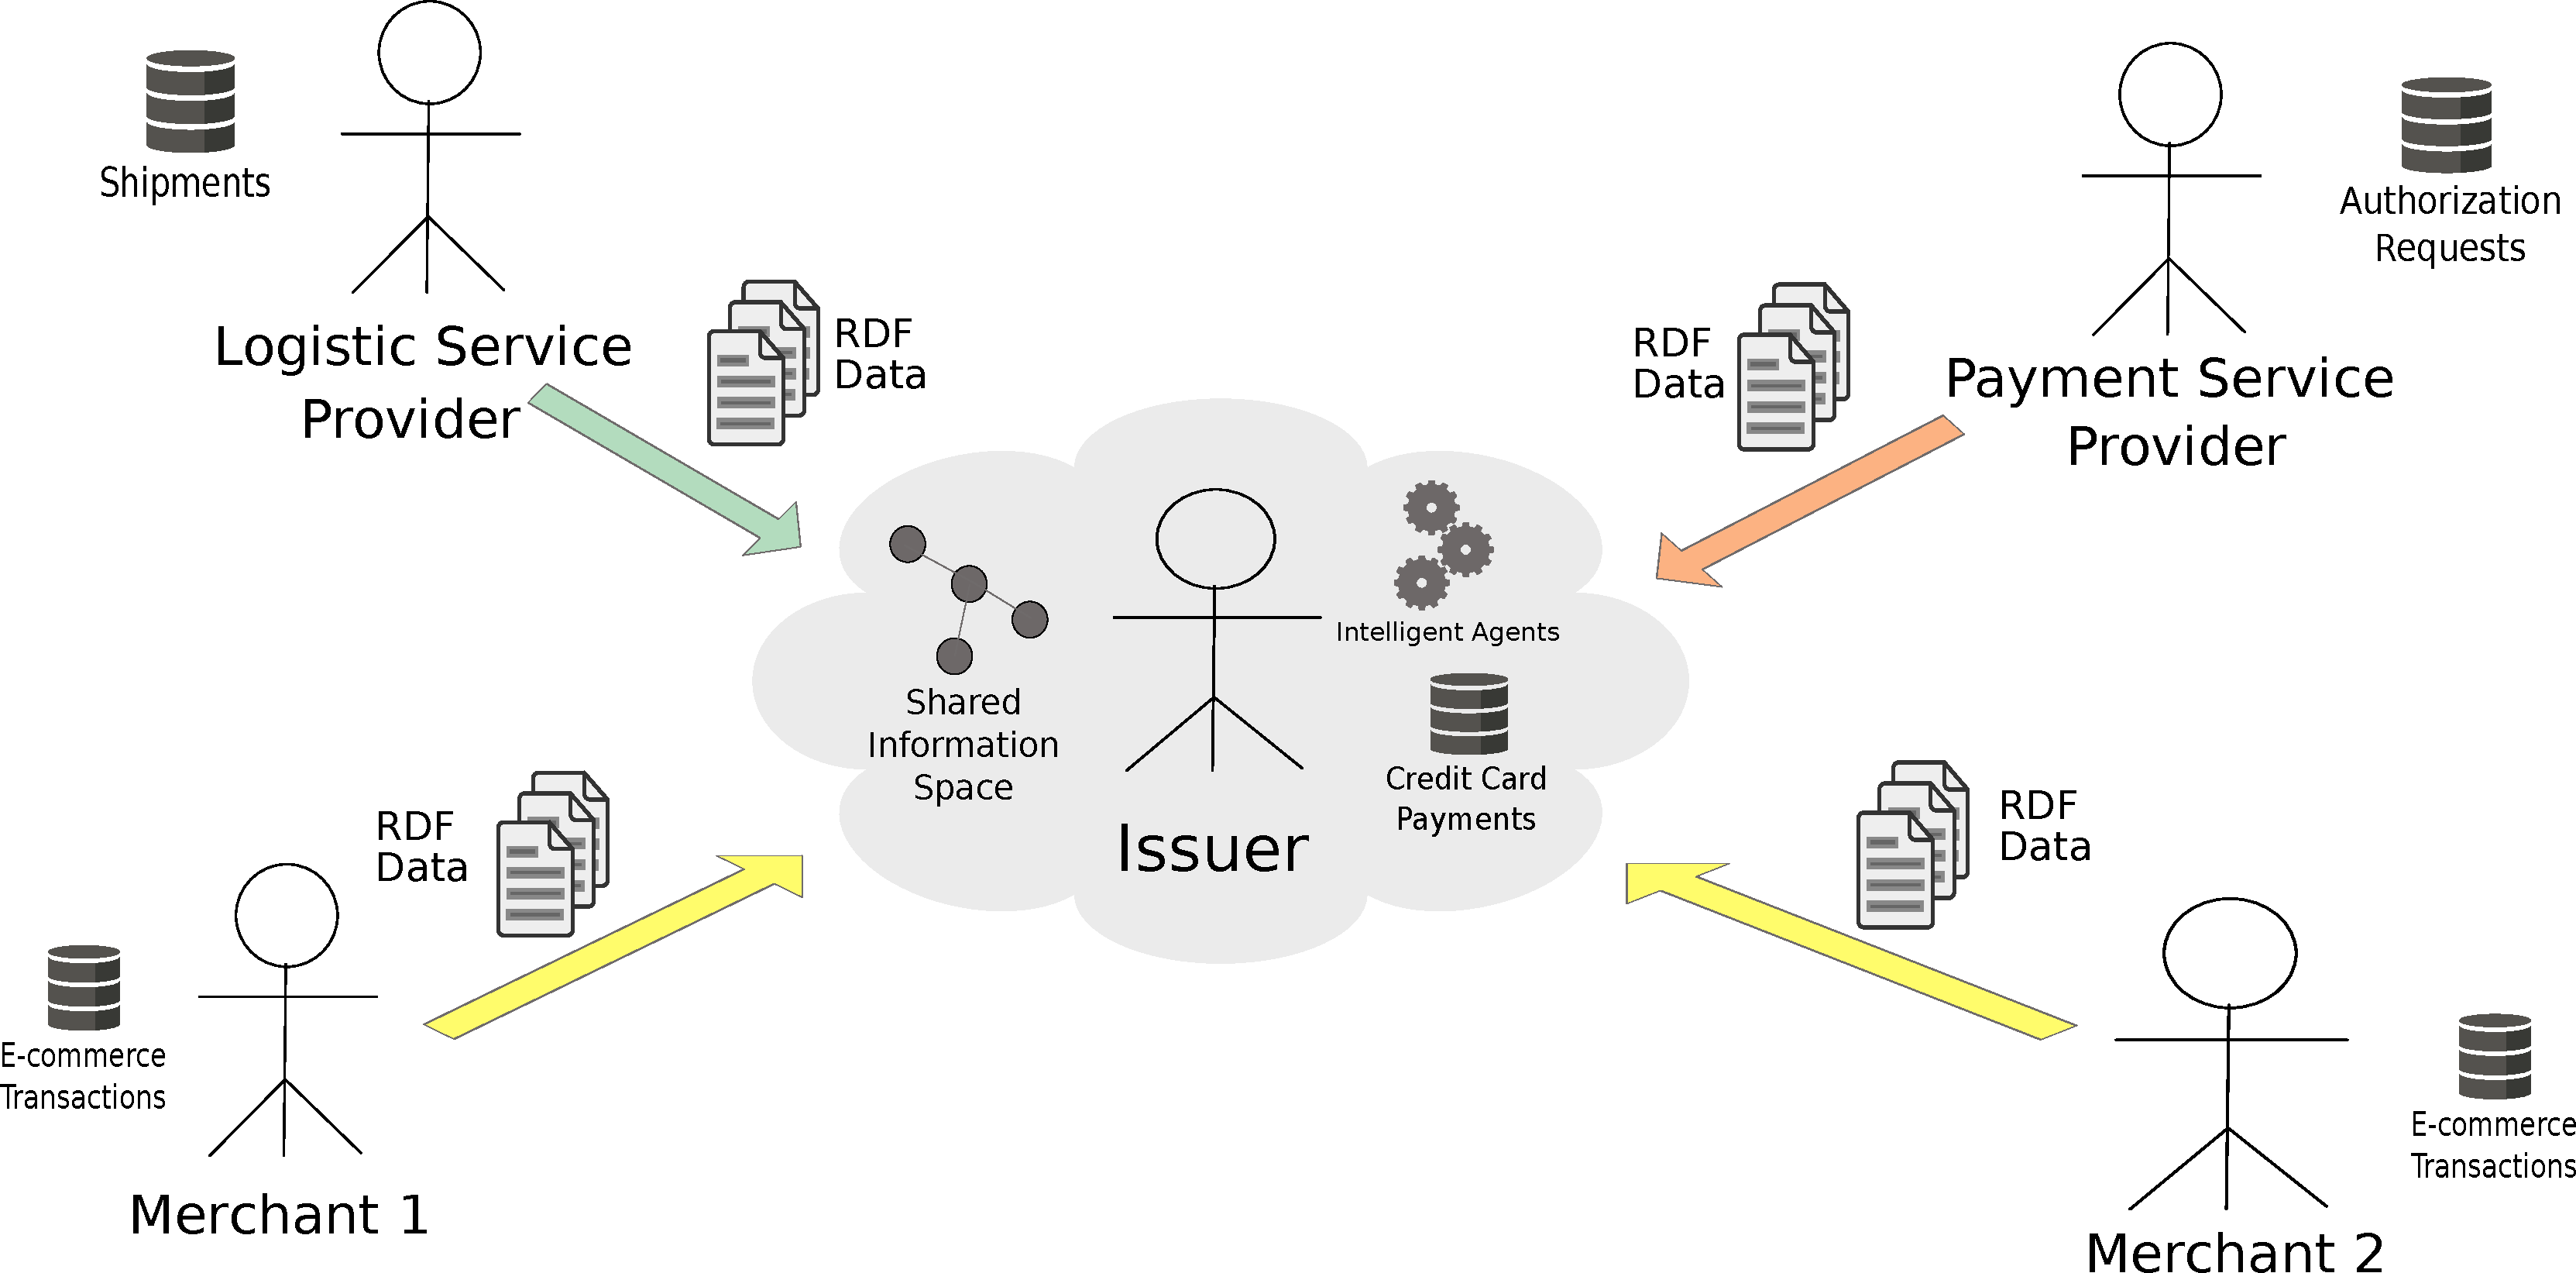
\includegraphics[width=0.9\columnwidth]{images/system_P2P_centralized.pdf}
	\caption{Collaborative system using a partially centralized \gls{P2P} architecture}
\label{fig:images_p2p_centralized}
\end{figure}


\subsection{Handling of privacy issues}
\label{subsec:p2p_partially_issuer_privacy}

One of the major concerns with the system architecture mentioned above is that the merchants, \gls{PSP}s and \gls{LSP}s have to hand over all of their relevant information to the issuer of a credit card for analysing the \gls{E-commerce} activities of a consumer. This can raise severe privacy issues, because an issuer will receive a lot of detailed order information from the other parties within this collaborative system. Issuers can not only use these information for validating the correctness of suspicious online transactions, but can also misuse them to build elaborate consumer profiles, which can directly influence the scoring of that consumer in the internal credit and risk rating systems of the issuers. \\

In addition to that, online merchants will likely not provide to much detail information about their sales and offerings in such a collaborative system, because direct competitors might also be involved in the \gls{E-commerce} fraud investigation. By sharing parts of the business relevant information, the merchants will raise the fear that their internal business processes, pricing structures, as well as customer loyalty activities get more transparent to their competitors, which might lead to a stronger competition afterwards. \\

During the design of the collaborative system a valuation of the shared information has to take place, which classify each of them based on the criteria: \@

\begin{itemize}
	\item Is the information really necessary to evaluate the \gls{E-commerce} transactions? Some of the order details from the merchants might not be required to analyse the transactions with the objective to find out about abnormal behaviours.
	\item Is the information worth protecting? Parts of the necessary information are sensitive information and should be protected against misuse.
\end{itemize}

Special considerations have to be taken for mandatory \emph{and} sensitive information. In that case, cryptographic algorithms such as hash functions (e.g.\ \gls{SHA-2}) can be used to anonymise the information. A hash function is working in one-direction only, and generates a unique hash value based on its input parameter. This hash value is different as soon as the input changes only slightly, and due to the mathematical algorithms used for computing it, a hash value can not be calculated back to the original input value of the hash function afterwards. \\

A valid use case for such a hashing of information is the e-mail address of a consumer. A plaintext e-mail address such as ``max.mustermann@web.de'' will always result in a \gls{SHA-2}56 based hash value of ``349124ca834949537d726da26dc029e593be72a8b00b81 c47124f5d009c9982b'' regardless of the stakeholder, who has originally computed it. That is an additional benefit of the usage of hash functions, because they still allow the information from different stakeholders to be linked together based on their unique hash values. \\

Another approach to protect sensitive information is to consolidate them in a broader context --- a process called data generalization. An example for that would be the item categories, which can be split up into multiple hierarchical layers to narrowly define the affiliations of items to certain product groups. Instead of exchanging item descriptions with the complete set of categories they belong to, merchants can just share items and their top n categories to obfuscate detailed information about the products bought by a consumer. The same approach will also work for location based information, in which the shared information will not contain the exact geographic position from the original data set, but use an approximation to it by stating locations on a broader scope (e.g.\ district, city or region) instead. \\

Based on these explanations the information, which is shared in the \gls{E-commerce} fraud investigation, can be classified into one of the following four quadrants, and should be handled as depicted in Figure~\ref{fig:images_handle_privacy_concerns}. \@

\begin{figure}[H]
	\centering
		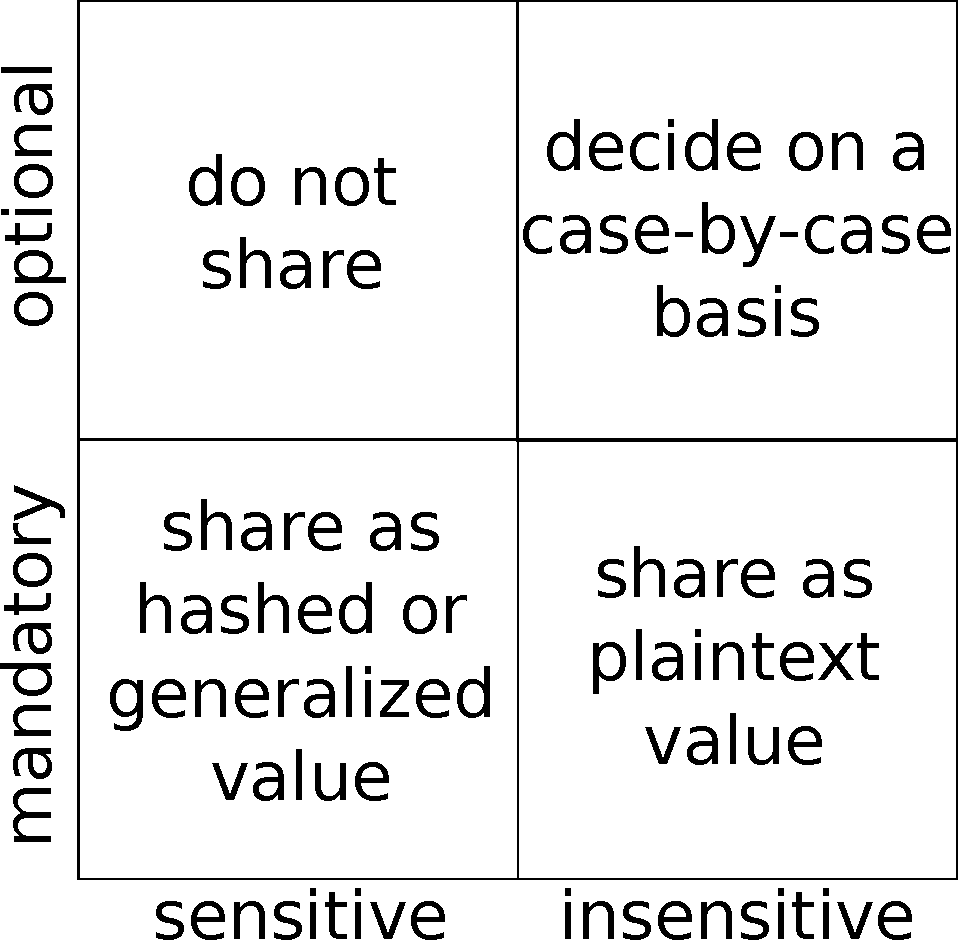
\includegraphics[width=0.5\columnwidth]{images/privacy_concerns.pdf}
	\caption{Privacy related classification of information in the collaborative system}
\label{fig:images_handle_privacy_concerns}
\end{figure}

% subsec p2p_partially_centralized_system

% section design_proposal (end)


% chapter design system (end)


% The counter for tables and figures are set back in order to start a new numeration per chapter
\setcounter{table}{1}
\setcounter{figure}{1}
  % Inclusion of the fith chapter
  %!TEX root = ../MasterThesis.tex

\chapter{Conclusion and Future Work} % (fold)
\label{cha:conclusion}

\section{Conclusion}
\label{sec:conclusion}

Initially, this Master thesis started with three fundamental assumptions: \@

\begin{enumerate}
	\item the use of an unsecure computer network to transfer credit card information in the \gls{E-commerce} scenario make them always subject to frauds and counterfeits,
	\item the existing technological solutions to detect and prevent them will not be able to cover 100\% due to the complexity and dynamics of the whole system, and
	\item the substantial analysis of any suspicious transaction is not taken place today due to the enormous effort and time needed to collect all required information manually
\end{enumerate}

As this Master thesis has pointed out in Chapter~\ref{cha:introduction} and Chapter~\ref{cha:context_analysis} the first and second premise has been seen a lot of research and development in recent years. But neither an industry-wide usage of the \gls{PCI/DSS} standards to securely process personal and payment-related information, nor the widely adoption of rule-based or score-based fraud prevention systems has been able to stop deceivers from cheating the \gls{E-commerce} system and bringing harm to the merchants and consumers alike. Whereas the Master thesis has shown the impact of \gls{E-commerce} frauds to the merchants, who are usually the ones that have to cover the losses, it also makes clear that any successful fraud attempt will reduce the thrust into the \gls{E-commerce} system, which is a substantial part of the global economics already. \\

Thus, bringing down the amount of fraudulent transactions in the system cannot be done with technology alone, but require a sharing of information between experts coming from various organizations. As the Master thesis explained in Section~\ref{subsec:e_commerce_fraud_handling} this consolidation of information about a suspicious transaction is currently not being done in-depth as this would require a lengthy manual communication and analyzation process by the investigator of an issuer or \gls{PSP}. This fact has lead to the third premise as well as to the hypothesis that the introduction of a collaborative system, which makes use of Semantic Web and peer-to-peer communication technologies to collect the information and know-how of the relevant stakeholders and link them together, can improve this siutation significantly. \\

As explained in Section~\ref{sec:system_approaches} existing approaches for integrating information from different sources are either to restrictive to work on a large scale (Web services), or are to open for the sharing of personal and payment-related information (Semantic Web). Therefore a new proposal for a collaborative system has been developed in Chapter~\ref{cha:system_concept} and Chapter~\ref{cha:system_design}, which uses suitable aspects from the Semantic Web standards as well as a secure \gls{P2P} communication network between the stakeholders for collaborating on \gls{E-commerce} fraud incidents. \\

Due to the fact that the information will be provided from dispersed organizations the proposed solution have to deal with differences in structure and wording of them. In these circumstances the \gls{W3C} standards such as \gls{RDF}, \gls{RDFS}, \gls{OWL} and \gls{SPARQL} show their full potential. As part of the Semantic Web initiative they already solve these issues on a global scale. Still, those standards only provide the basics for integrating distributed information. Additional steps are required to build intelligent applications on top of them. In Chapter~\ref{cha:system_concept} the Master thesis showed that the information has to be combined into a graph-oriented representation of the \gls{E-commerce} activities done with a credit card recently. Based on the initial clustering of order details by merchant a subsequent mapping and linking of the information has to be done to be able to cluster the transactions on different aspects with the objective to find abnormal activities.

\section{Towards a decentralized \gls{P2P} system}
\label{sec:p2p_decentralized_system}

In the decentralized P2P system architecture each node is equal and keeps their local data ready for analysis if the node is online. If the issuer will have to figure out, whether a transaction is fraudulent or not, she is going to send out various queries to all the available nodes in the P2P cluster asking for certain information that help investigating the case. The other nodes, whose reside on each stakeholder involved, will answering the queries based on the common Schema.org data mapping shown above and send back the results to the issuer bank. The issuer will collect all the results from the various parties and combine them to be able to analyze the issue and come up with a conclusion. The main benefit of this architecture is, that there is no need to duplicate the data from the other stakeholders to the issuer. Due to this it can also be a better suited solution if data sharing faces restrictions due to law or regulations. On the other hand this architecture will depend on the nodes being online all the time so the issuer can query for information at any time. So this works only in synchronous communication mode. Additionally there are efforts spread around all the stakeholders to set up and maintain a system for secure data querying functionality, please see Figure~\ref{fig:images_p2p_decentralized}.

\begin{figure}[H]
	\centering
		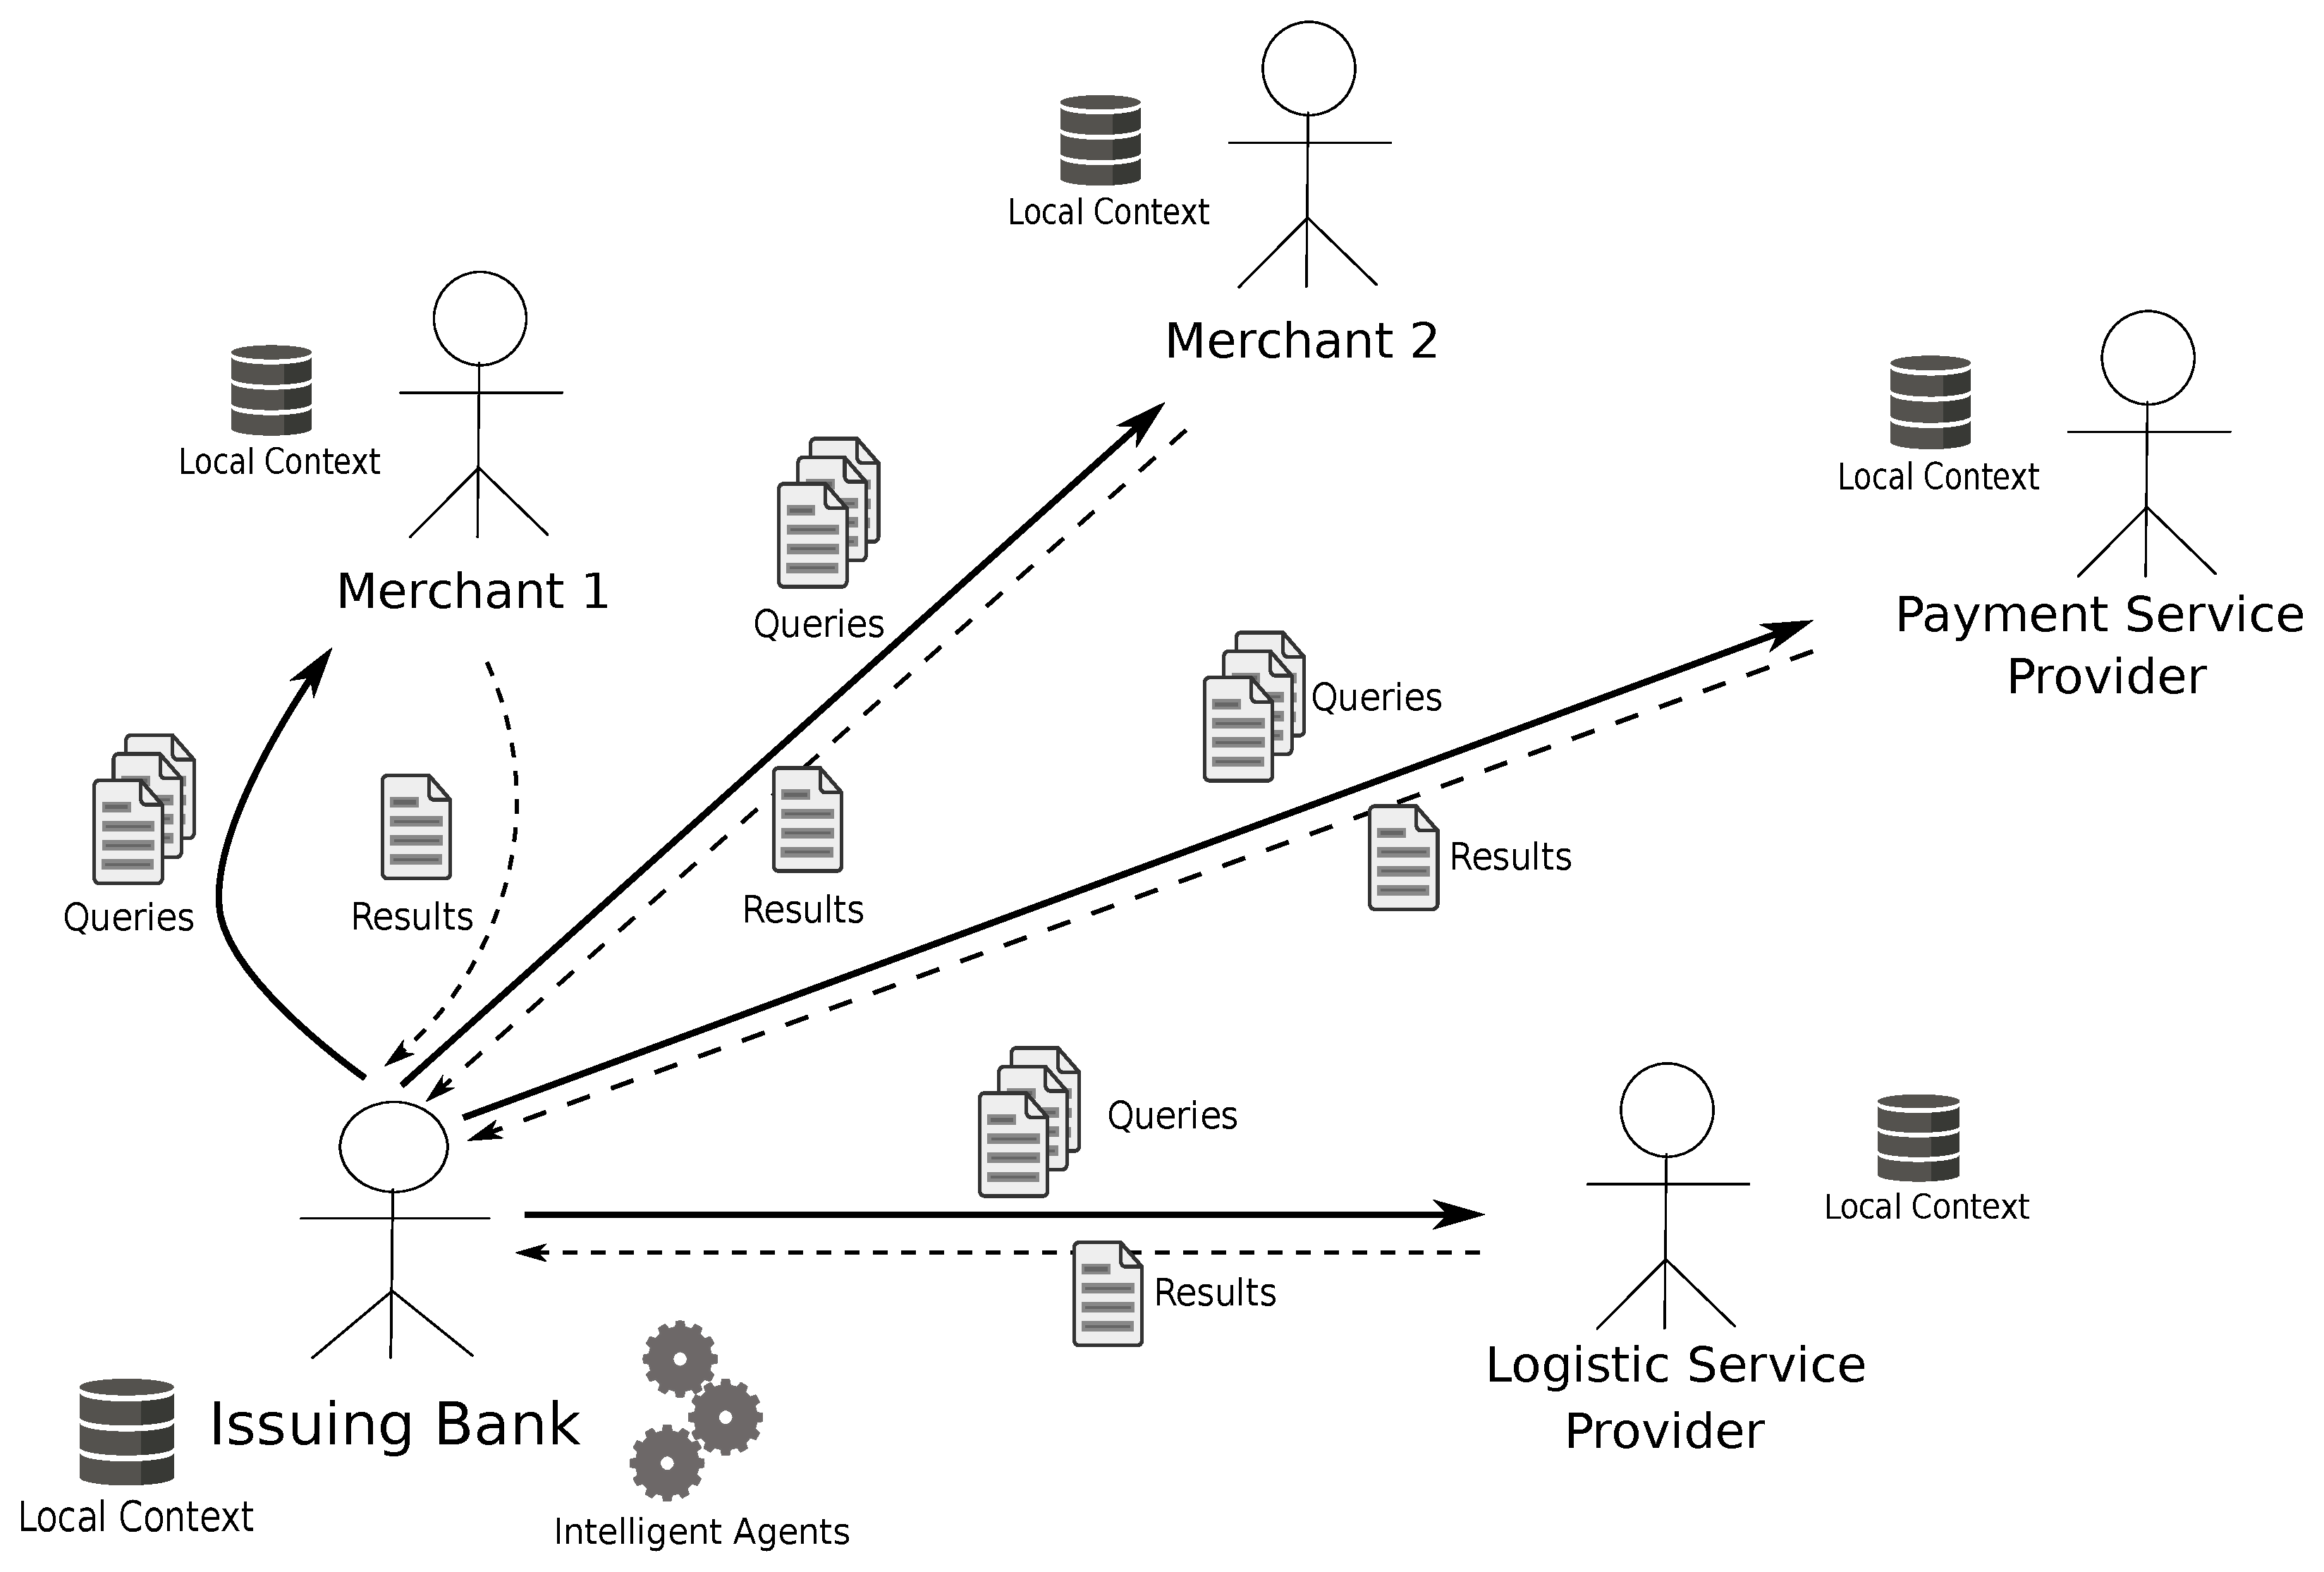
\includegraphics[width=0.9\columnwidth]{images/system_P2P_decentralized.pdf}
	\caption{Decentralized \gls{P2P} system architecture}
\label{fig:images_p2p_decentralized}
\end{figure}

% sec p2p_decentralized_system

% chapter conclusion (end)


\singlespacing
	%!TEX root = ../MasterThesis.tex

% Creates list of figures
\listoffigures
% Inserts the row "`List of figures"' as a chapter in the table of content
\addcontentsline{toc}{chapter}{List of figures}

% Creates list of tables
\listoftables
% Inserts the row "`List of tables"' as a chapter in the table of content
\addcontentsline{toc}{chapter}{List of tables}

% Creates list of listings
\listoflistings
% Inserts the row "`List of tables"' as a chapter in the table of content
\addcontentsline{toc}{chapter}{List of listings}

% insert glossary items
\printglossary[style=long]
\addcontentsline{toc}{chapter}{Glossary}

% Changes Style of references
% \bibliographystyle{geralpha}
% Creates references list by the use of the file "`references.bib"'
\bibliography{MasterThesis}
% Inserts the row "`Bilbiography"' as a chapter in the table of content
\addcontentsline{toc}{chapter}{Bibliography}

	%!TEX root = ../TemplateMasterThesis.tex

\chapter*{Declaration in lieu of oath}
\addcontentsline{toc}{chapter}{Declaration in lieu of oath}

I hereby declare that this master thesis was independently composed and authored by myself. \\ \\


All content and ideas drawn directly or indirectly from external sources are indicated as such. All sources and materials that have been used are referred to in this thesis. \\ \\


The thesis has not been submitted to any other examining body and has not been published.

\vspace{1.5cm}
\\
Place, date and signature of student
\vspace{3cm}
\\
Jane Doe



% chapter declaration_in_lieu_of_oath (end)

%=== Final part =====================================================
\backmatter
% \pagenumbering{Roman}

	%!TEX root = ../MasterThesis.tex

% \begin{appendices}
% \adjustmtc
% \renewcommand{\appendixname}{APPENDIX}
% \renewcommand{\appendixtocname}{\appendixname}
% \addappheadtotoc

% \part*{Appendix}

% \end{appendices}

	\include{chapter/affidavit}

\end{document}
